\documentclass[../PianoProgetto.tex]{subfiles}
\begin{document}
	\section{Preventivo}
		\subsection{Dettaglio fasi}
			\subsubsection{Fase A}
				\paragraph{Suddivisione del lavoro}\
	\begin{table}[H]
		%\centering
		\begin{tabularx}{\textwidth}{l  * {6}{C}  c}
			\toprule
			\textbf{Nominativo} & \textbf{Rp} & \textbf{Am} & \textbf{Pt} 
						& \textbf{An} & \textbf{Pm} & \textbf{Ve} & \textbf{Ore totali} \\
			\midrule
			Andrighetto Cristian & 0 & 15 &	0 &	10 & 0 & 15 & 40 \\
			%\midrule
			Bicego Eduard & 4 & 10 & 0 & 0 & 0 & 26 & 40 \\
			%\midrule
			Castello Davide &	0 &	20 & 0 & 10 & 0 & 10 & 40 \\
			%\midrule
			Conti Oscar Elia & 0 & 20 &	0 &	15 & 0 & 5 & 40 \\
			%\midrule
			Tavella Federico &	17 & 2 & 0 & 21 & 0 & 0 & 40 \\
			%\midrule
			Tombolato Andrea & 12 & 5 &	0 &	20 & 0 & 3 & 40 \\
			%\midrule
			Zanella Marco & 0 & 15 & 0 & 10 & 0 & 15 & 40 \\
			\midrule			
			\textbf{Ore Totali Ruolo} & 33 & 87 & 0 & 86 &	0 &	74 & 280 \\
			\bottomrule
		\end{tabularx}
		\caption{Fase A - Suddivisione delle ore di lavoro}
		\label{tab:faseA_ore}
	\end{table}
	\vfill
	\begin{figure}[H]
		\centering
		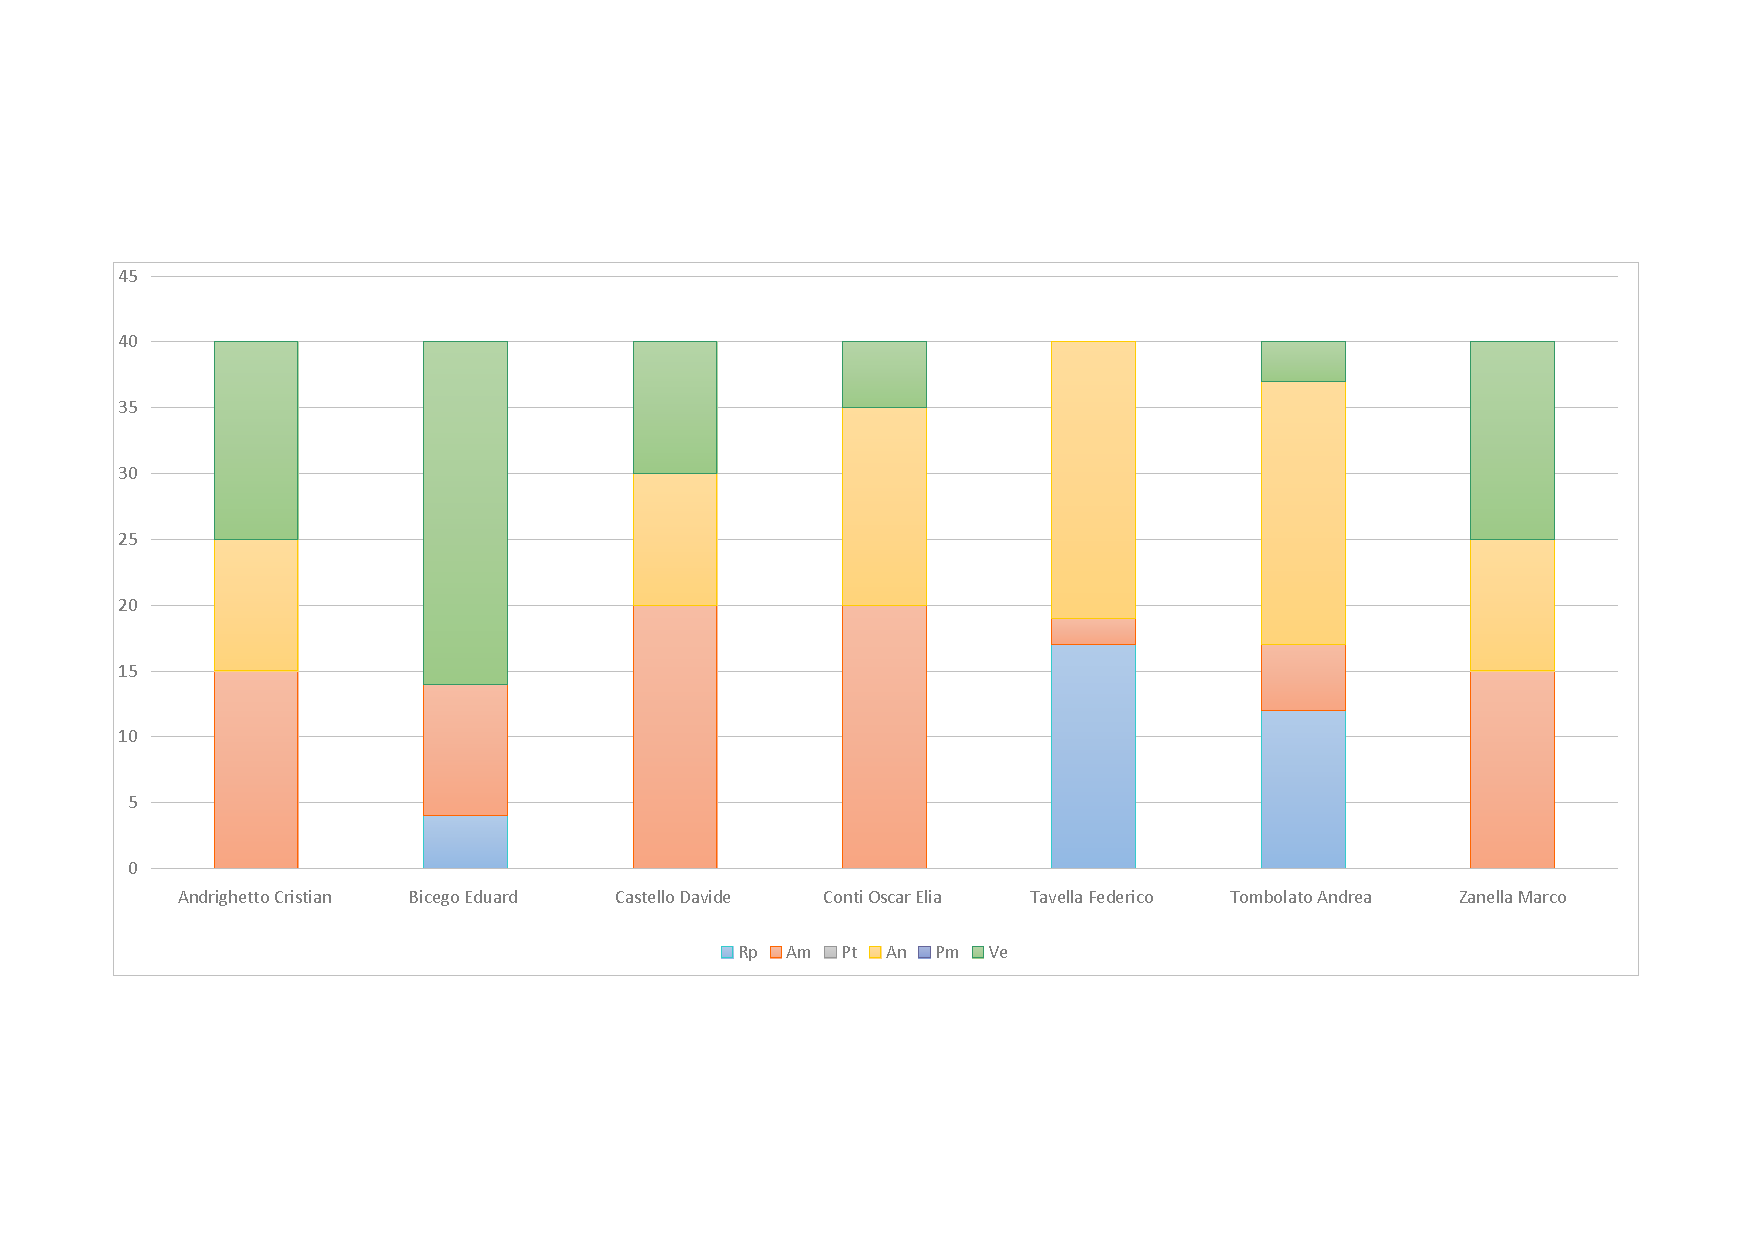
\includegraphics[width=\textwidth, trim=2cm 4cm 2cm 4cm]{grafici/A/A-ore-persona}
			\caption{Fase A - Riassunto}
		\label{fig:BarChart-faseA_ore}
	\end{figure}	
	
\newpage
	\vfill	
	\paragraph{Prospetto economico}\
	
	\begin{table}[H]
		\centering
		\begin{tabular}{l * {2}{c}}
			\toprule
			\textbf{Ruolo} & \textbf{Ore} & \textbf{Costo (\euro{})} \\
			\midrule
			Responsabile &	33 &  990,00 \\
			%\midrule
			Amministratore & 87 &  1.740,00 \\
			%\midrule
			Progettista & 0 & 0,00 \\
			%\midrule
			Analista & 86 & 2,150,00 \\
			%\midrule
			Programmatore & 0 & 0,00 \\
			%\midrule
			Verificatore & 74 & 1.110,00 \\
			\midrule		
			\textbf{Totale} & 280 & 5.990,00 \\
			\bottomrule	
		\end{tabular}
		\caption{Fase A - Costo per ruolo}
		\label{tab:faseA_costo}
	\end{table}

	\begin{figure}[H]
		\centering
		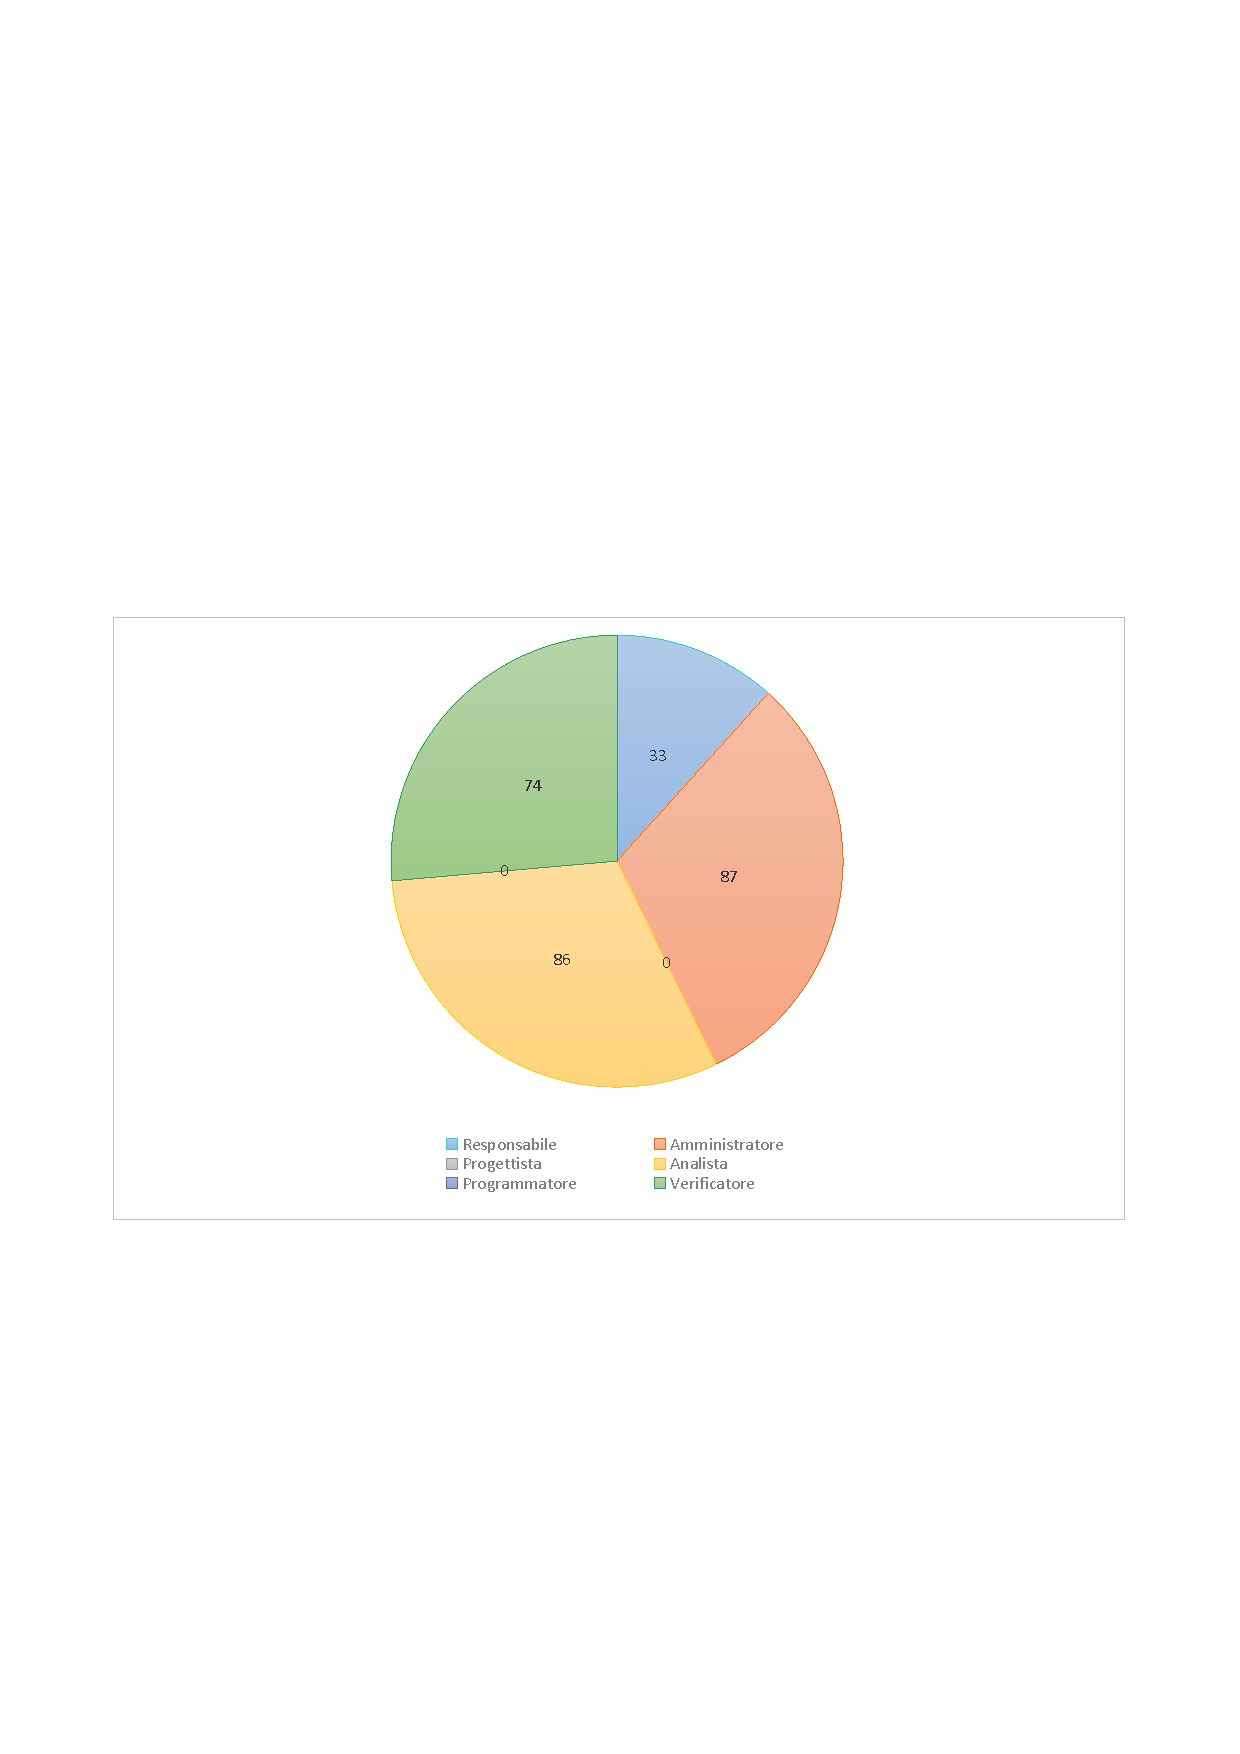
\includegraphics[width=0.93\textwidth , trim=1.5cm 9cm 1.5cm 9cm]{grafici/A/A-ore-ruolo}
			\caption{Fase A - Ore per ruolo}
		\label{fig:CircleChart-faseA_ore_r}
	\end{figure}
	\vfill
	\newpage
	\vfill	
	\begin{figure}[H]
		\centering
		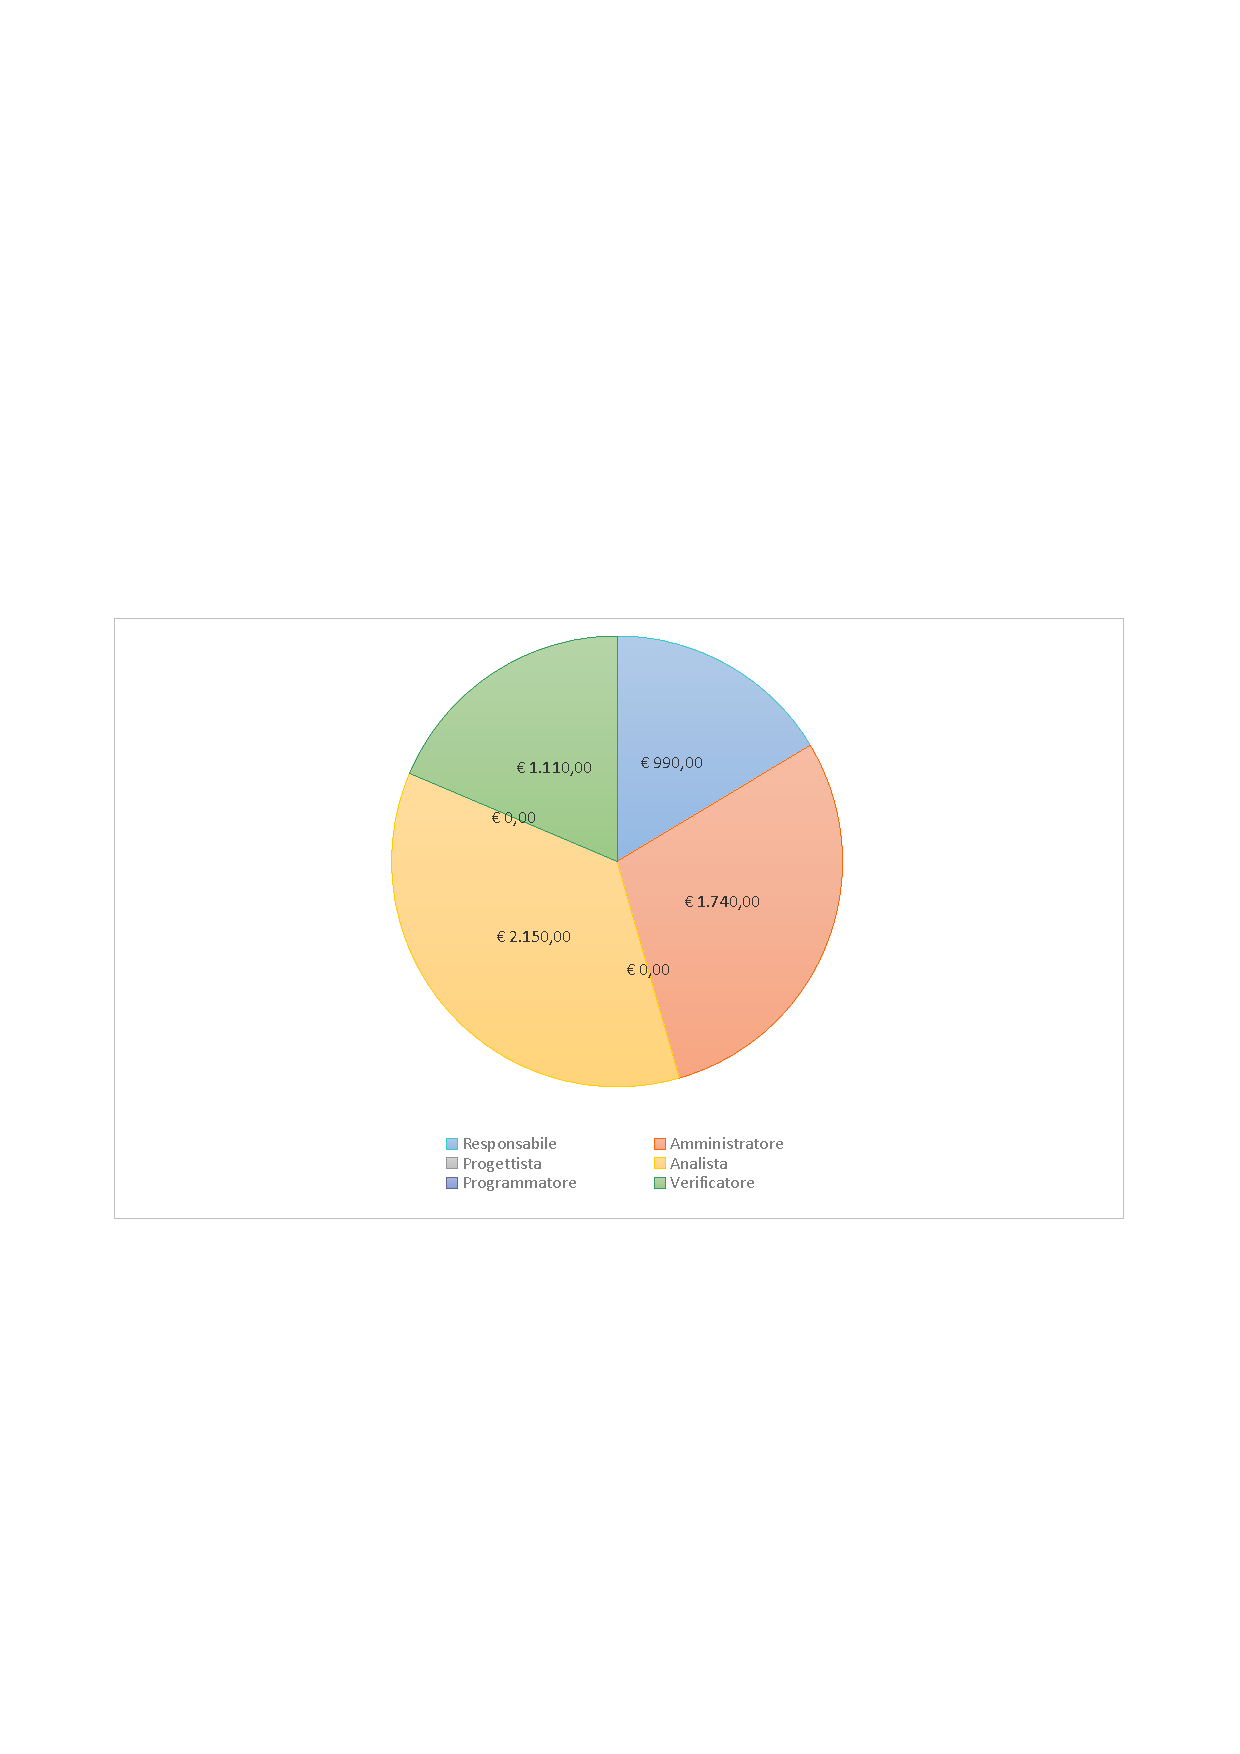
\includegraphics[width=0.93\textwidth , trim=1.5cm 9cm 1.5cm 9cm]{grafici/A/A-costo}
			\caption{Fase A - Costo per ruolo}
		\label{fig:CircleChart-faseA_costo}
	\end{figure}
\vfill
	
	\subsubsection{Fase AD}
				\paragraph{Suddivisione del lavoro}\
				
	\begin{table}[H]
		%\centering
		\begin{tabularx}{\textwidth}{l  * {6}{C}  c}
			\toprule
			\textbf{Nominativo} & \textbf{Rp} & \textbf{Am} & \textbf{Pt} 
						& \textbf{An} & \textbf{Pm} & \textbf{Ve} & \textbf{Ore totali} \\
			\midrule
			Andrighetto Cristian & 9 & 3 &	0 &	0 & 0 & 0 & 12 \\
			%\midrule
			Bicego Eduard & 0 & 6 & 0 & 0 & 0 & 6 & 12 \\
			%\midrule
			Castello Davide & 0 & 5 & 0 & 0 & 0 & 6 & 11 \\
			%\midrule
			Conti Oscar Elia & 0 & 0 &	0 &	6 & 0 & 6 & 12 \\
			%\midrule
			Tavella Federico &	0 & 0 & 0 & 5 & 0 & 7 & 12 \\
			%\midrule
			Tombolato Andrea & 0 & 0 &	0 &	4 & 0 & 7 & 11 \\
			%\midrule
			Zanella Marco & 0 & 0 & 0 & 5 & 0 & 6 & 11 \\
			\midrule			
			\textbf{Ore Totali Ruolo} & 9 & 14 & 0 & 20 & 0 & 38 & 81 \\
			\bottomrule
		\end{tabularx}	
		\caption{Fase AD - Suddivisione delle ore di lavoro}
		\label{tab:faseAD_ore}	
	\end{table}
\vfill
\newpage
\vfill
	
	\begin{figure}[H]
		\centering
		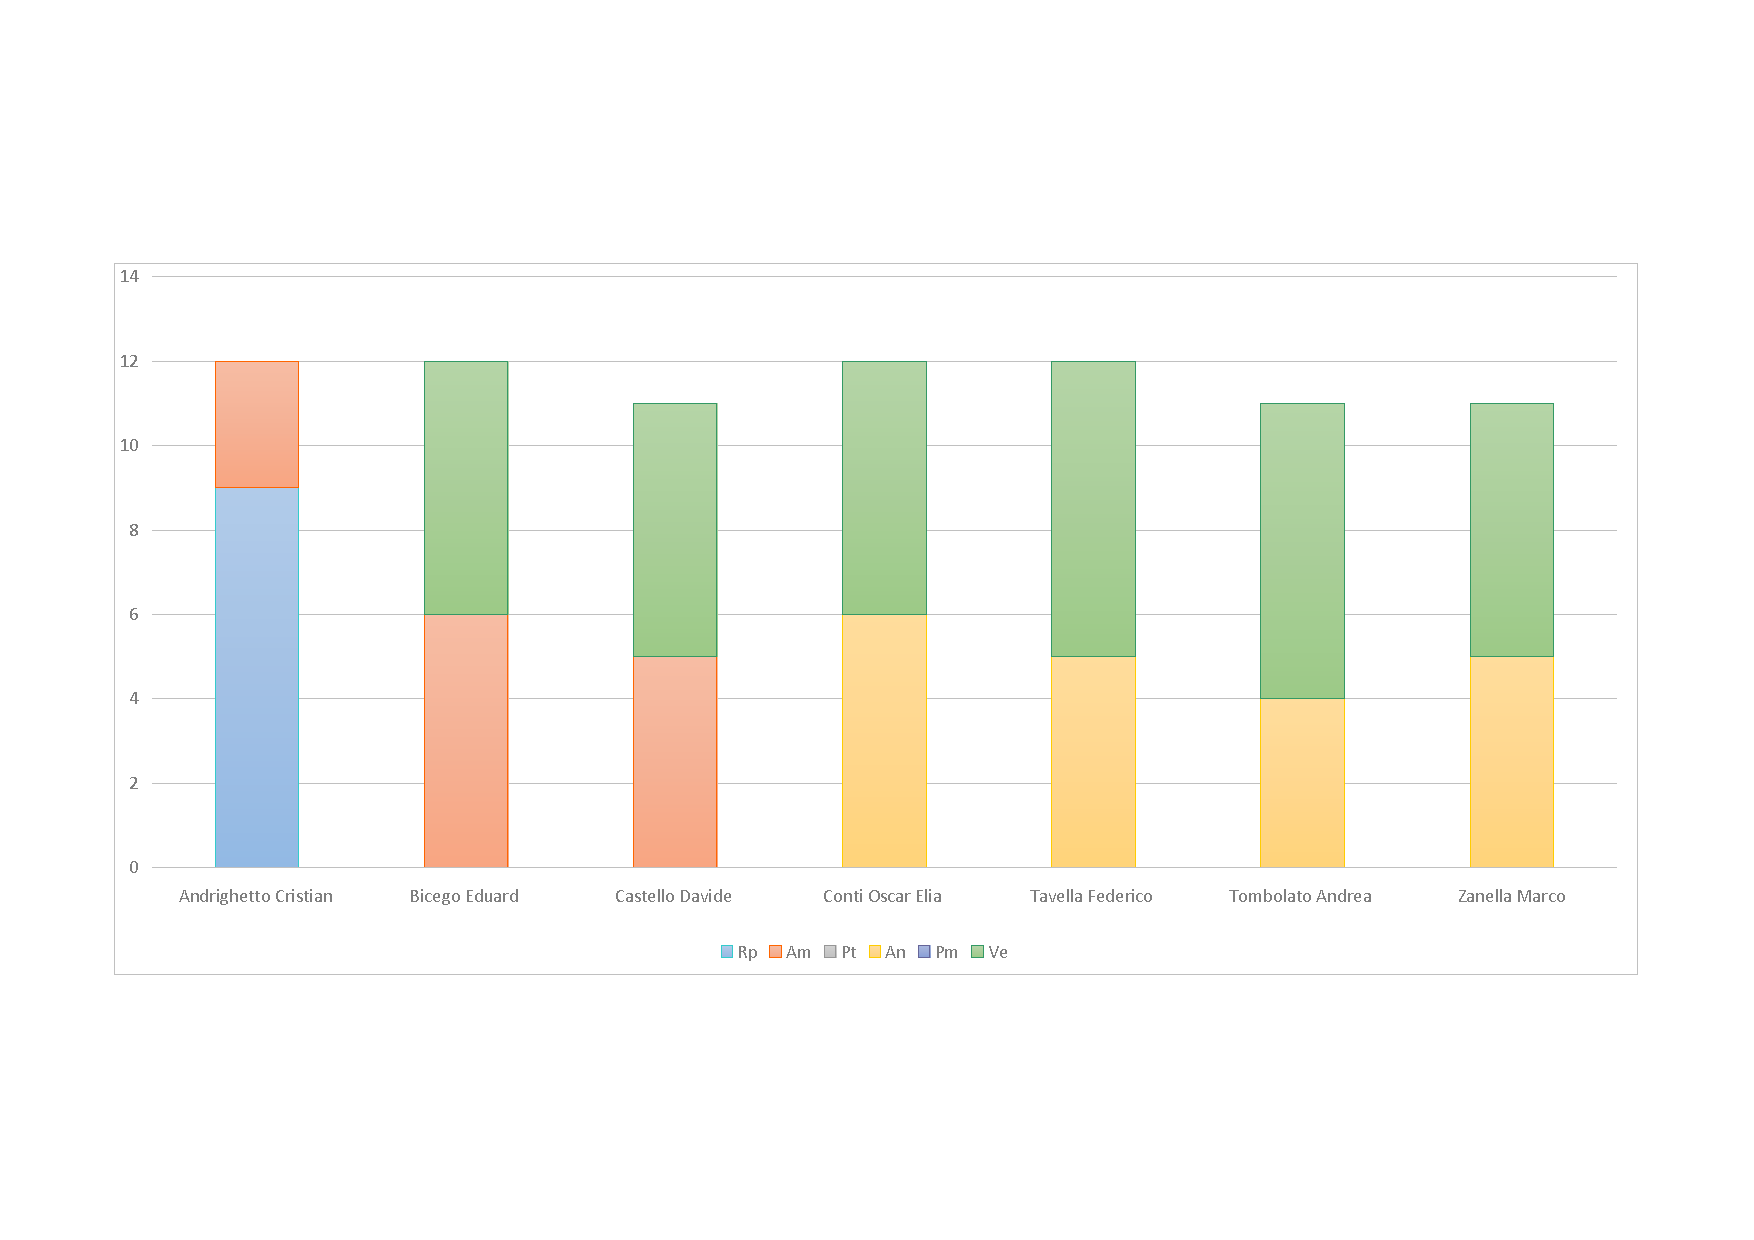
\includegraphics[width=\textwidth , trim=2cm 4cm 2cm 4cm]{grafici/AD/AD-ore-persona}
			\caption{Fase AD - Riassunto}
		\label{fig:BarChart-faseAD_ore}
	\end{figure}
	
\vfill
	
	\paragraph{Prospetto economico}\
	
					\begin{table}[H]
		\centering
	
		\begin{tabular}{l * {2}{c}}
			\toprule
			\textbf{Ruolo} & \textbf{Ore} & \textbf{Costo (\euro{})} \\
			\midrule
			Responsabile &	9 & 270,00 \\
			%\midrule
			Amministratore & 14 & 280,00 \\
			%\midrule
			Progettista & 0 & 0,00 \\
			%\midrule
			Analista & 20 & 500,00 \\
			%\midrule
			Programmatore & 0 & 0,00 \\
			%\midrule
			Verificatore & 38 & 570,00 \\
			\midrule		
			\textbf{Totale} & 81 & 1.620,00 \\
			\bottomrule 
		\end{tabular}
		\caption{Fase AD - Costo per ruolo}
		\label{tab:faseAD_costo}
	\end{table}
\vfill
\newpage
	
	\begin{figure}[H]
		\centering
		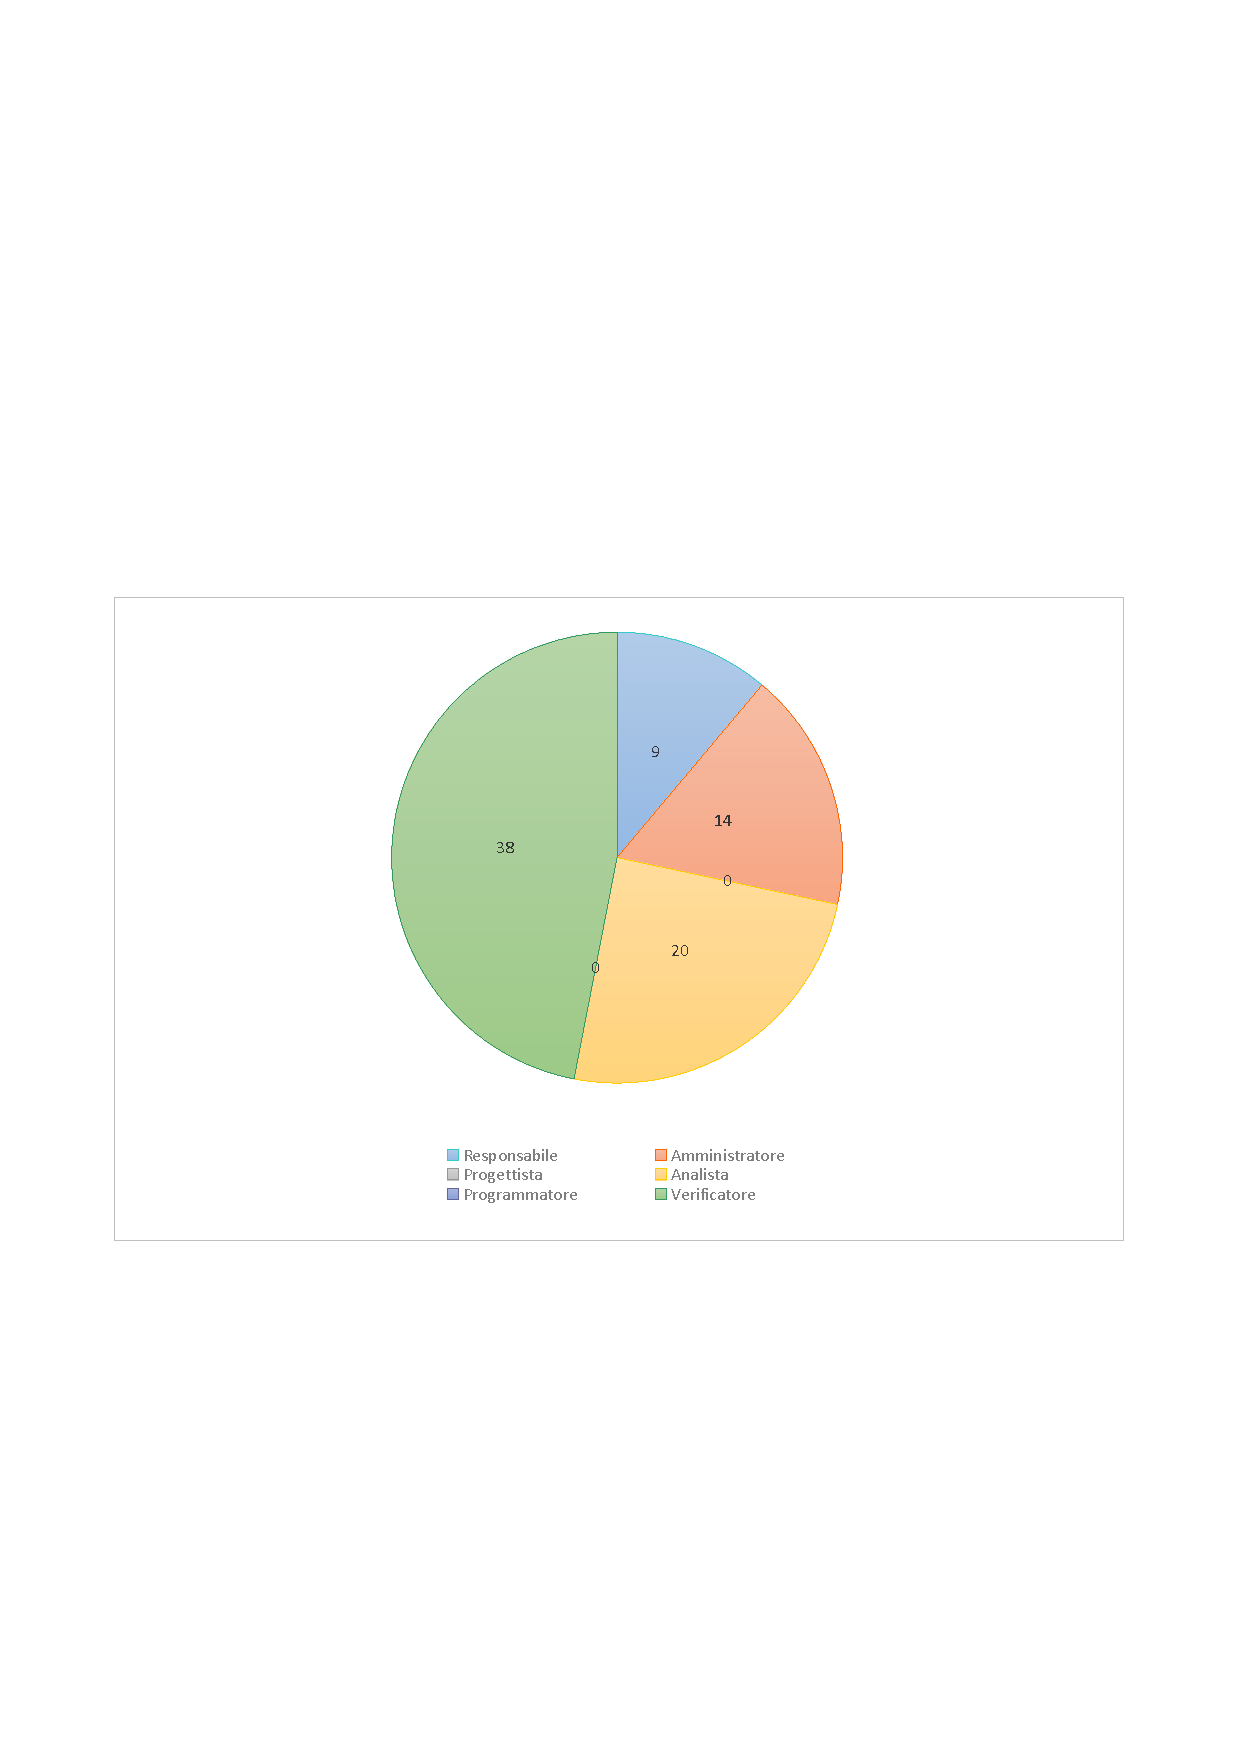
\includegraphics[width=0.93\textwidth , trim=1.5cm 9cm 1.5cm 9cm]{grafici/AD/AD-ore-ruolo}
			\caption{Fase AD - Ore per ruolo}
		\label{fig:CircleChart-faseAD_ore_r}
	\end{figure}
\vfill
	\begin{figure}[H]
		\centering
		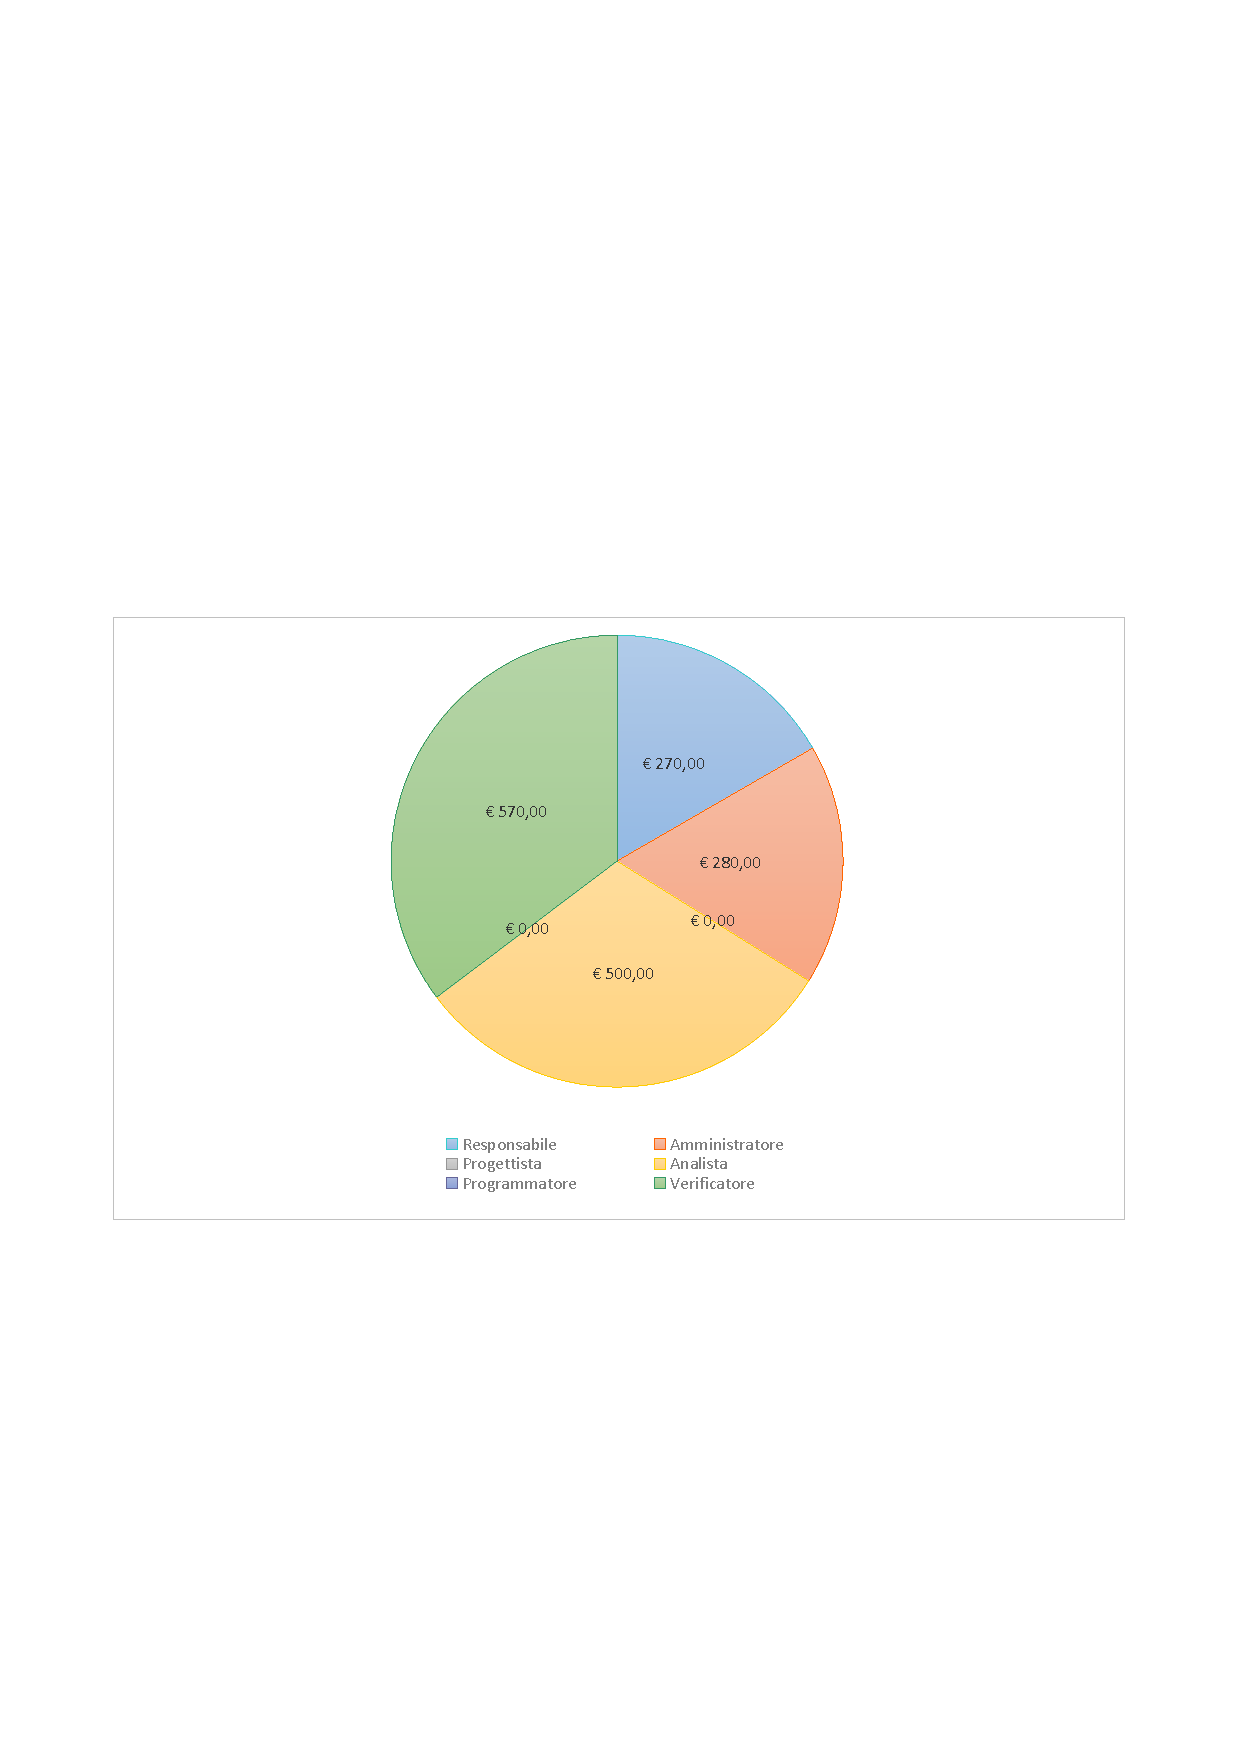
\includegraphics[width=0.93\textwidth , trim=1.5cm 9cm 1.5cm 9cm]{grafici/AD/AD-costo}
			\caption{Fase AD - Costo per ruolo}
		\label{fig:CircleChart-faseAD_costo}
	\end{figure}
\vfill		
\newpage	
	\subsubsection{Fase PA}
				\paragraph{Suddivisione del lavoro}\
						
	\begin{table}[H]
		\centering
	
		\begin{tabularx}{\textwidth}{l  * {6}{C}  c}
			\toprule
			\textbf{Nominativo} & \textbf{Rp} & \textbf{Am} & \textbf{Pt} 
						& \textbf{An} & \textbf{Pm} & \textbf{Ve} & \textbf{Ore totali} \\
			\midrule
			Andrighetto Cristian  & 0 & 0 & 15 & 8 & 0 & 0 & 23 \\
			Bicego Eduard  & 0 & 0 & 0 & 18 & 0 & 6 & 24 \\
			Castello Davide  & 0 & 0 & 0 & 26 & 0 & 2 & 28 \\
			Conti Oscar Elia  & 0 & 0 & 9 & 10 & 0 & 5 & 24 \\
			Tavella Federico  & 0 & 9 & 13 & 0 & 0 & 0 & 22 \\
			Tombolato Andrea  & 0 & 10 & 8 & 0 & 0 & 5 & 23 \\
			Zanella Marco & 10 & 0 & 0 & 13 & 0 & 0 & 23 \\
			\midrule
			\textbf{Ore Totali Ruolo} & 10 & 19 & 45 & 75 & 0 & 18 & 167 \\
			\bottomrule
		\end{tabularx}
		\caption{Fase PA - Suddivisione delle ore di lavoro}
		\label{tab:fasePA_ore}
	\end{table}
\vfill	
	
	\begin{figure}[H]
		\centering
		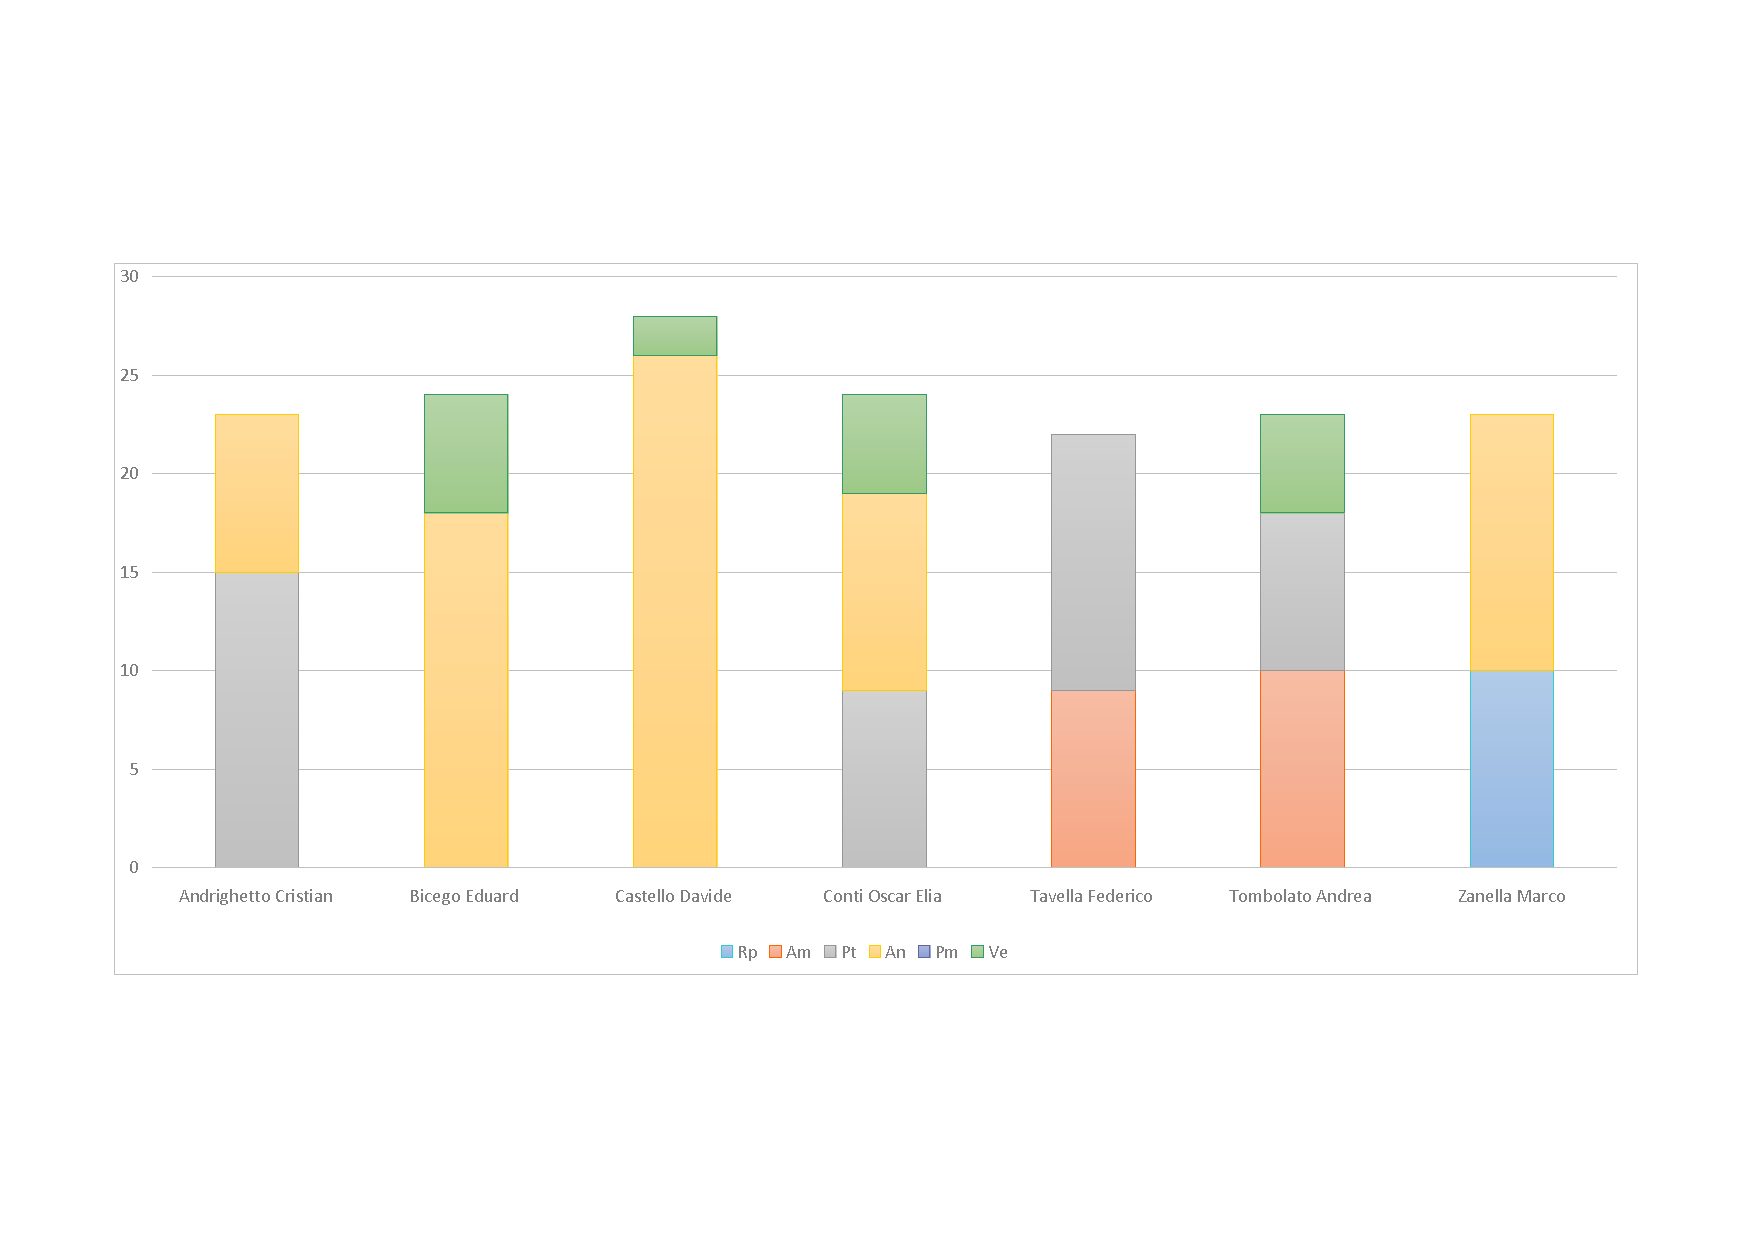
\includegraphics[width=\textwidth , trim=2cm 4cm 2cm 4cm]{grafici/PA/PA-ore-persona}
			\caption{Fase PA - Riassunto}
		\label{fig:BarChart-fasePA_ore}
	\end{figure}
\vfill	
\newpage
	
	\paragraph{Prospetto economico}\
					
	\begin{table}[H]
		\centering
	
		\begin{tabular}{l * {2}{c}}
			\toprule
			\textbf{Ruolo} & \textbf{Ore} & \textbf{Costo (\euro{})} \\
			\midrule
			Responsabile & 10    & 300,00 \\
			Amministratore  & 19    & 380,00 \\
			Progettista  & 45    & 990,00 \\
			Analista & 75    & 1.875,00 \\
			Programmatore  & 0    & 0,00 \\
			Verificatore  & 18    & 270,00 \\
			\midrule
			\textbf{Totale}  & 167   & 3.815,00 \\
			\bottomrule
		\end{tabular}
		\caption{Fase PA - Costo per ruolo}
		\label{tab:fasePA_costo}
	\end{table}
\vfill	
	
	\begin{figure}[H]
		\centering
		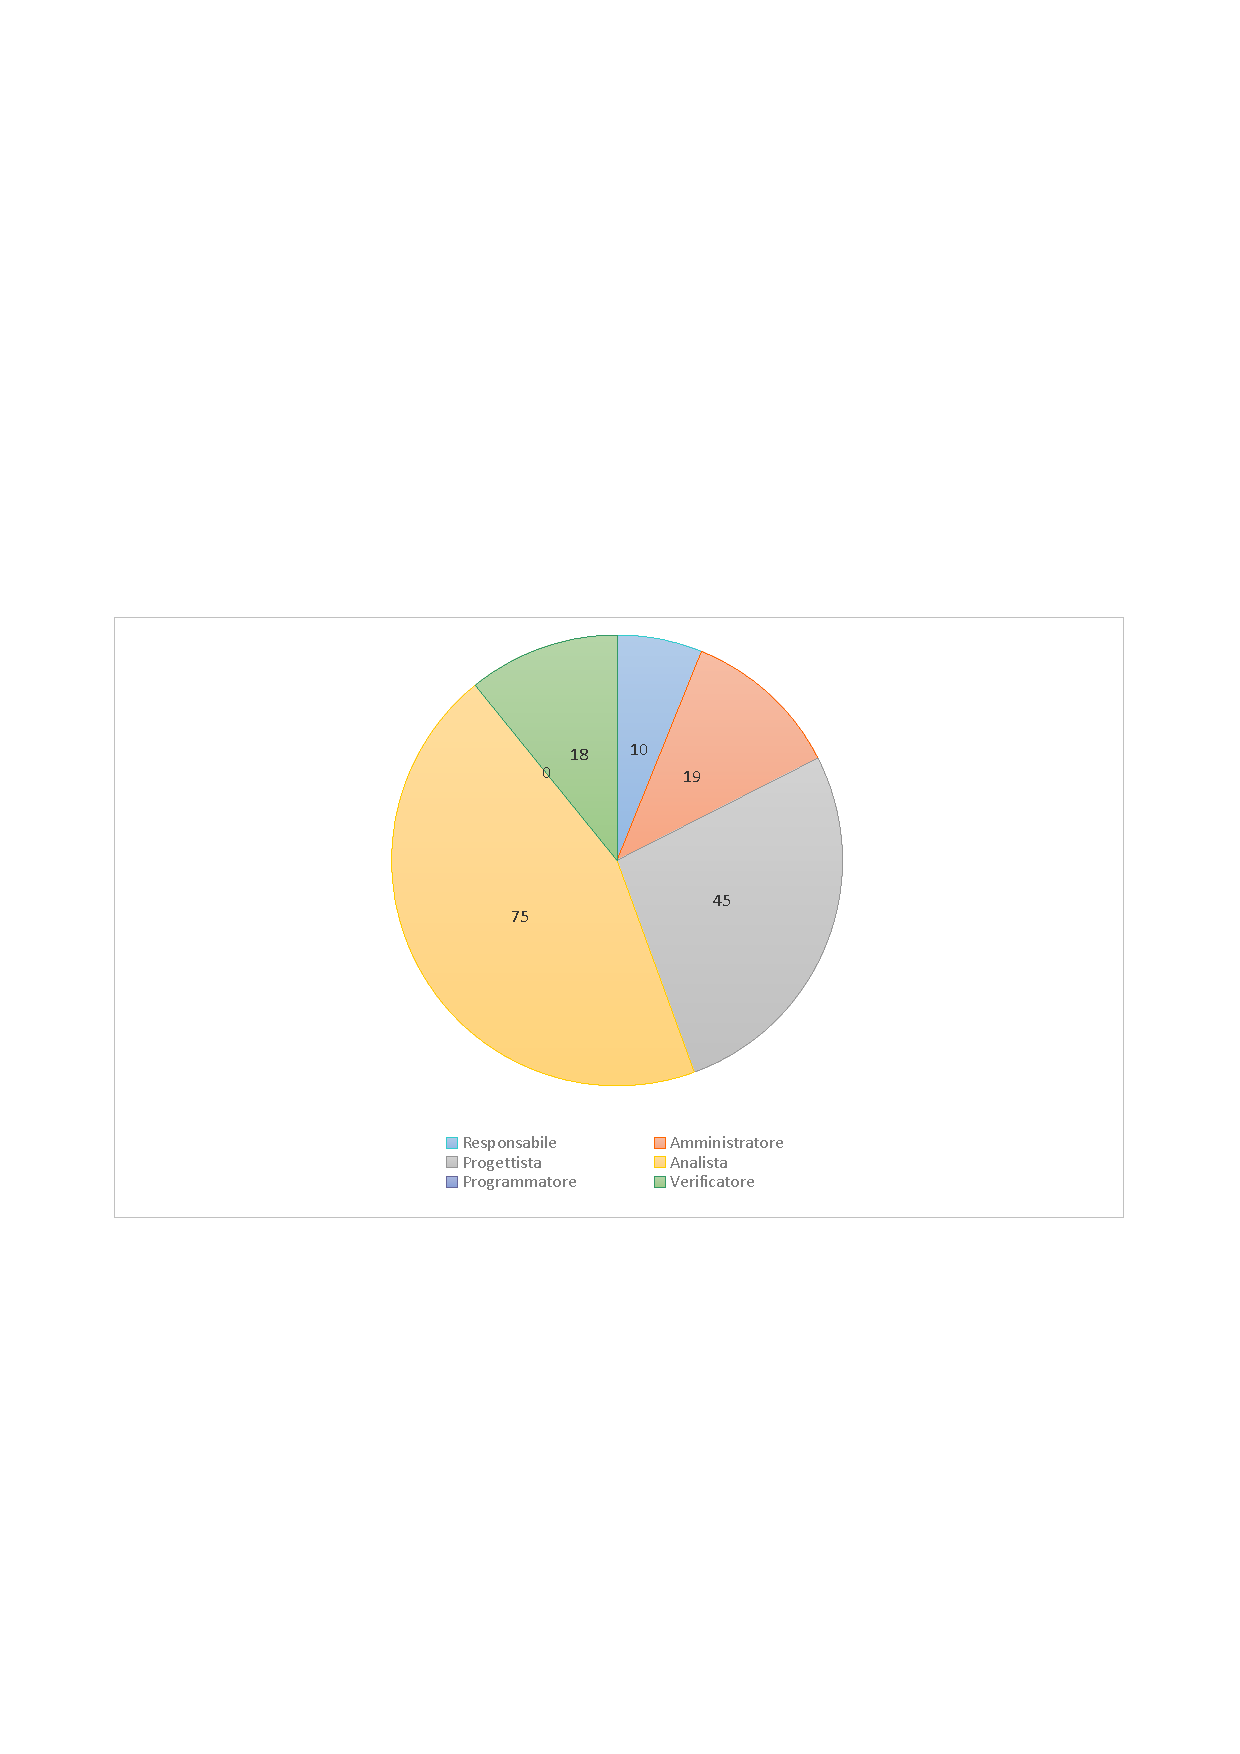
\includegraphics[width=0.93\textwidth , trim=1.5cm 9cm 1.5cm 9cm]{grafici/PA/PA-ore-ruolo}
			\caption{Fase PA - Ore per ruolo}
		\label{fig:CircleChart-fasePA_ore_r}
	\end{figure}
\vfill	
\newpage
\vfill
	\begin{figure}[H]
		\centering
		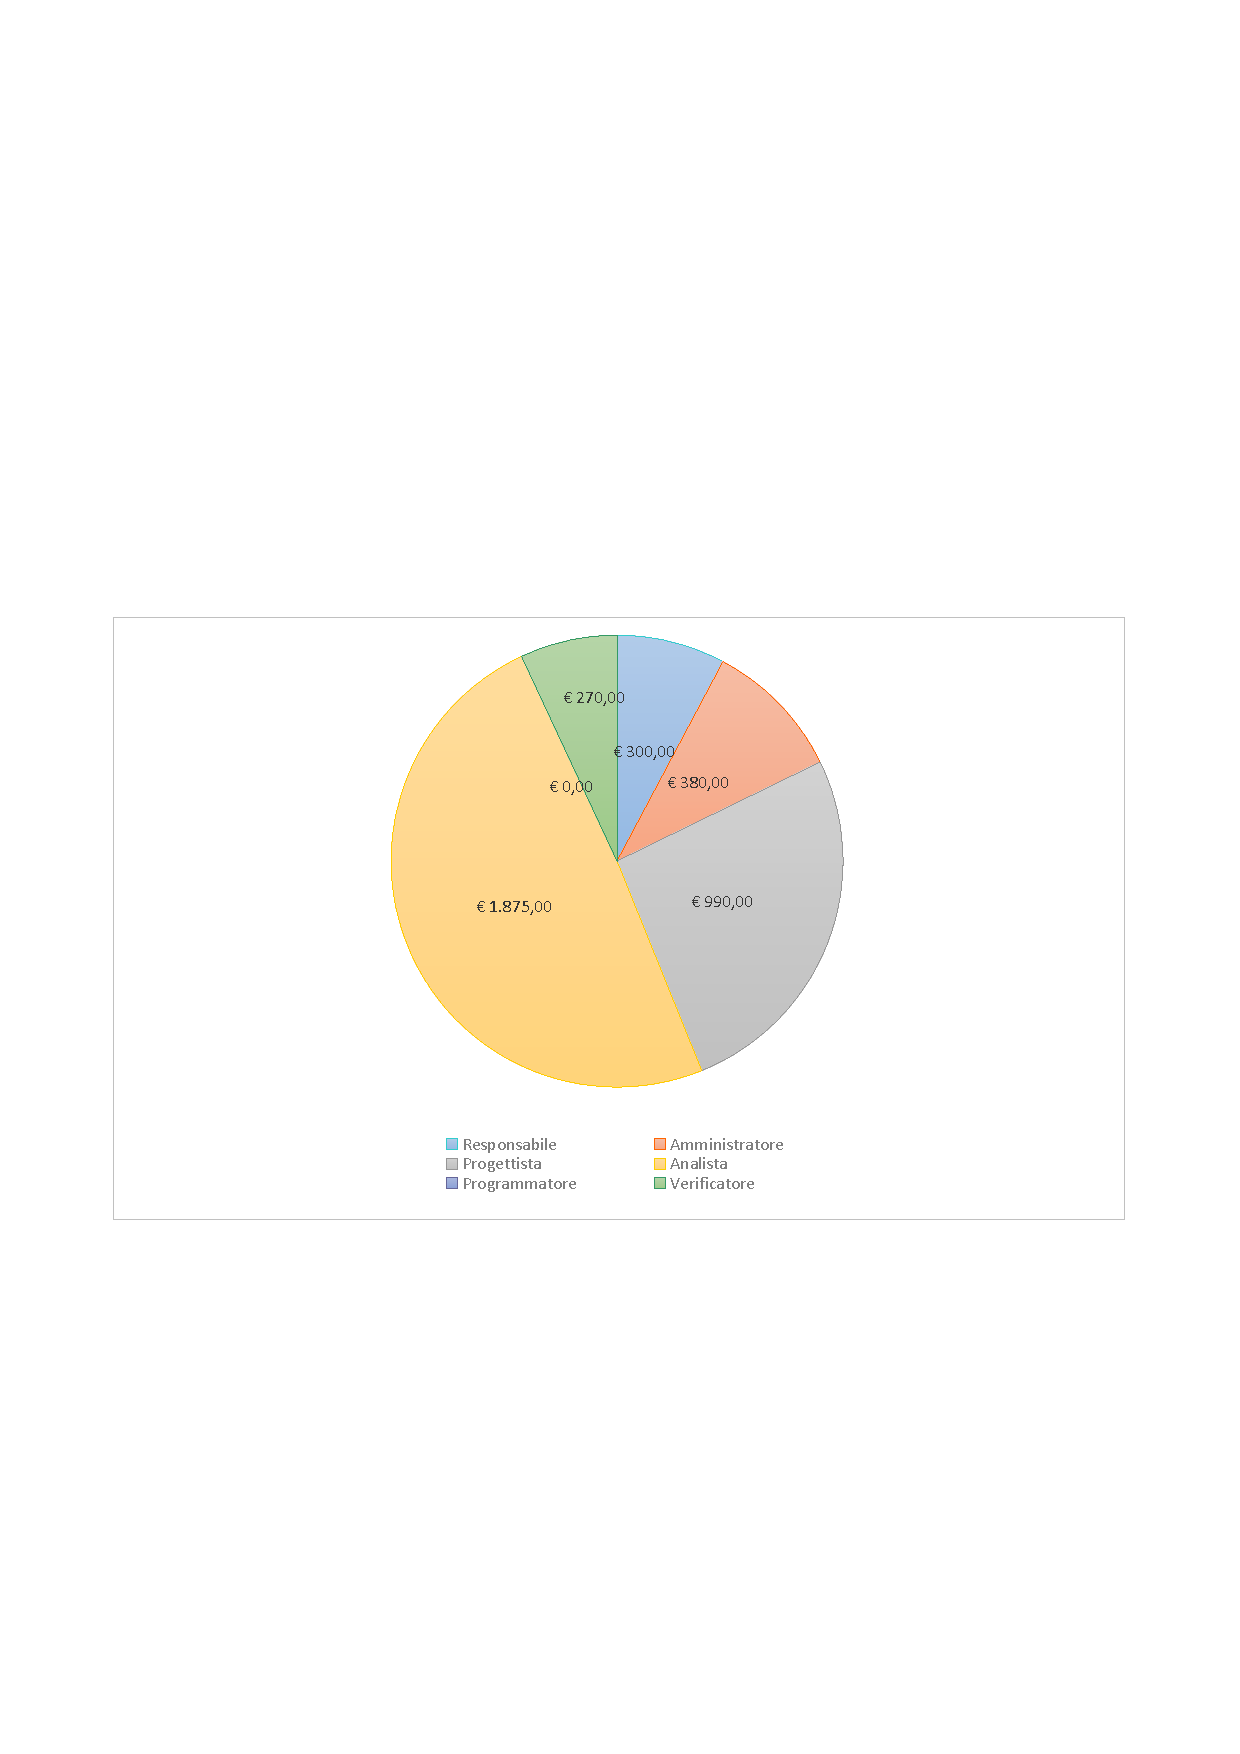
\includegraphics[width=0.93\textwidth , trim=1.5cm 9cm 1.5cm 9cm]{grafici/PA/PA-costo}
			\caption{Fase PA - Costo per ruolo}
		\label{fig:CircleChart-fasePA_costo}
	\end{figure}	
\vfill	
	\subsubsection{Fase PDROB}
				\paragraph{Suddivisione del lavoro}\
					
	
	\begin{table}[H]
		%\centering
	
		\begin{tabularx}{\textwidth}{l  * {6}{C}  c}
			\toprule
			\textbf{Nominativo} & \textbf{Rp} & \textbf{Am} & \textbf{Pt} 
						& \textbf{An} & \textbf{Pm} & \textbf{Ve} & \textbf{Ore totali} \\
			\midrule
			Andrighetto Cristian  & 0 & 0 & 0 & 17 & 0 & 11 & 28 \\
			Bicego Eduard  & 0 & 0 & 17 & 0 & 9 & 0 & 26 \\
			Castello Davide  & 0 & 5 & 19 & 0 & 0 & 0 & 24 \\
			Conti Oscar Elia  & 10 & 0 & 10 & 0 & 3 & 0 & 23 \\
			Tavella Federico  & 10 & 0 & 0 & 11 & 7 & 0 & 28 \\
			Tombolato Andrea  & 0 & 0 & 8 & 0 & 13 & 5 & 26 \\
			Zanella Marco & 0 & 0 & 8 & 0 & 12 & 4 & 24 \\
			\midrule			
			\textbf{Ore Totali Ruolo}& 20 & 5 & 62 & 28 & 44 & 20 & 179 \\
			\bottomrule	
		\end{tabularx}
		\caption{Fase PDROB - Suddivisione delle ore di lavoro}
		\label{tab:fasePDROB_ore}
	\end{table}
\vfill
\newpage
\vfill	
		
	\begin{figure}[H]
		\centering
		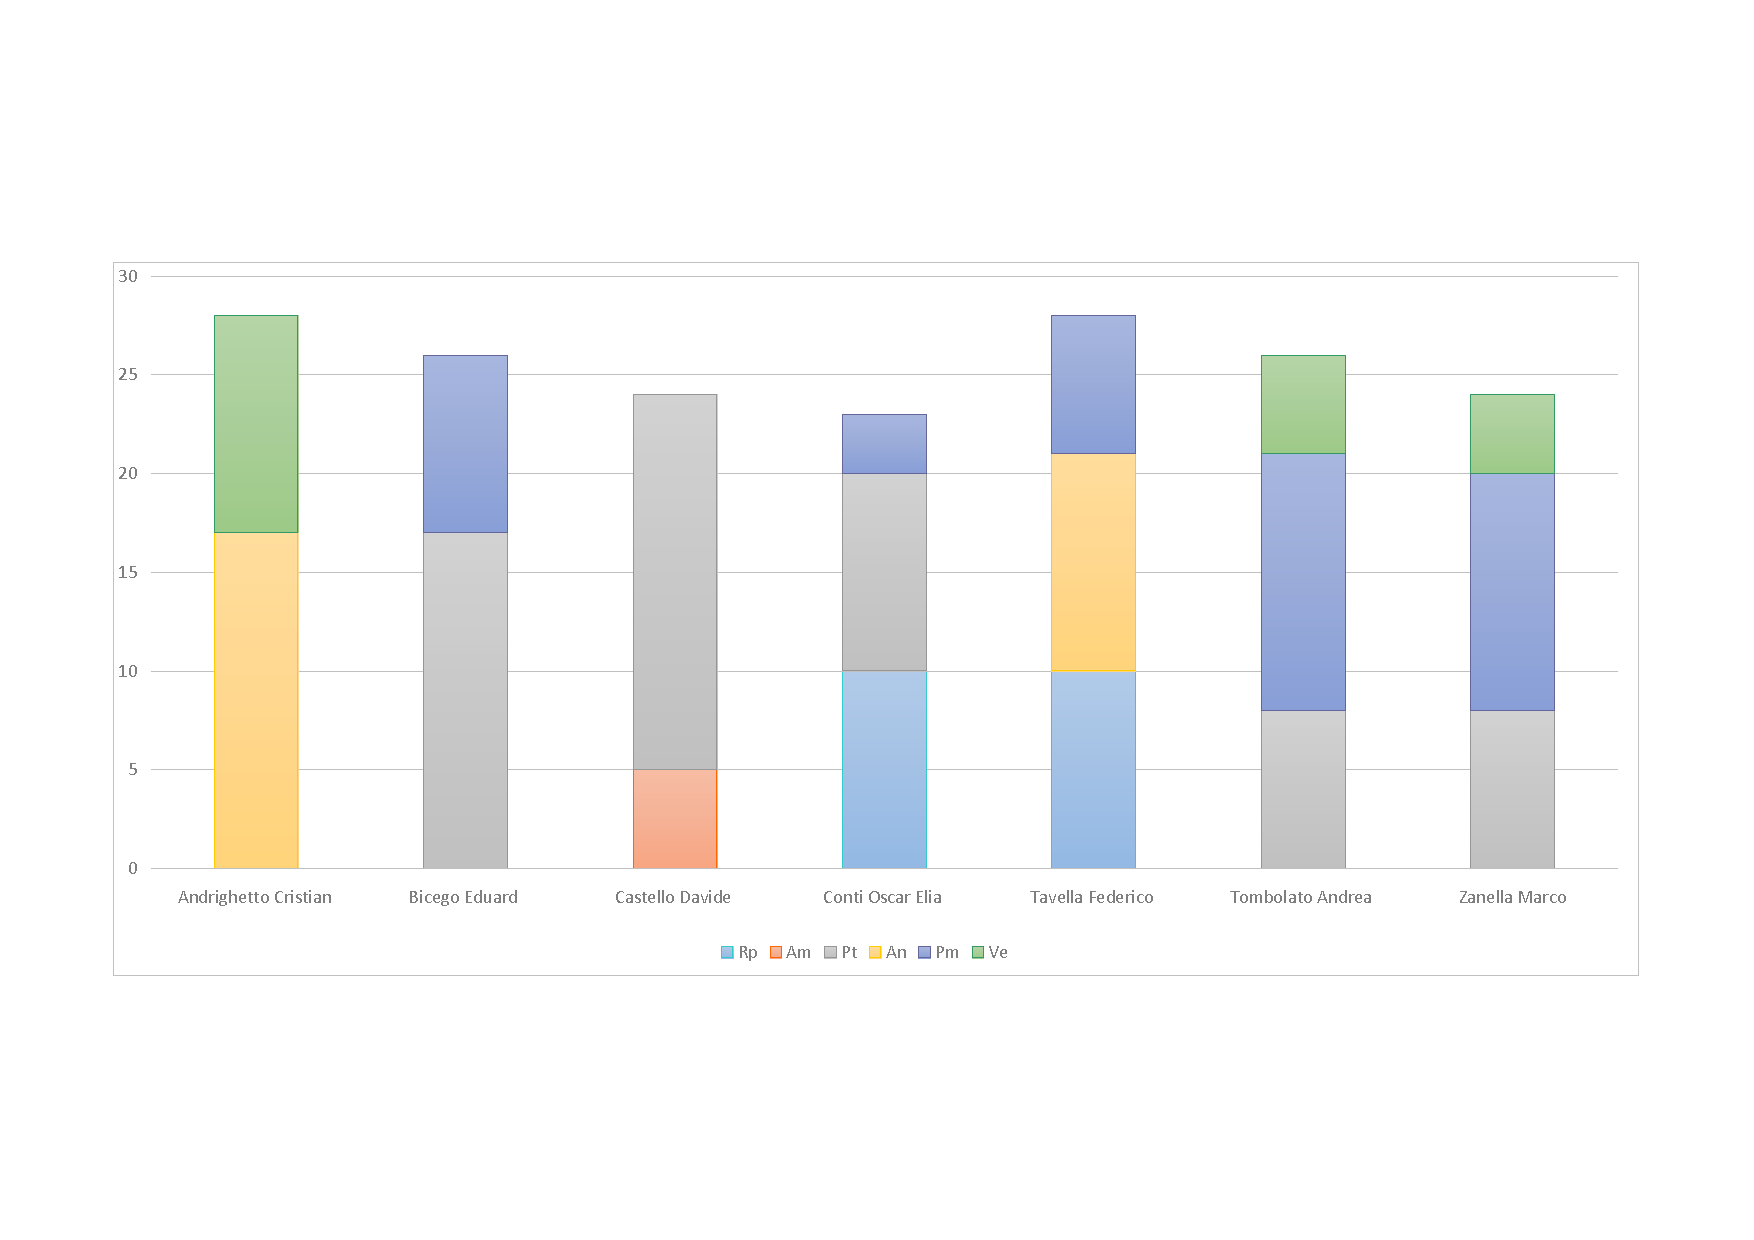
\includegraphics[width=\textwidth , trim=2cm 4cm 2cm 4cm]{grafici/PDROB/PDROB-ore-persona}
			\caption{Fase PDROB - Riassunto}
		\label{fig:BarChart-fasePDROB_ore}
	\end{figure}
\vfill	
	\paragraph{Prospetto economico}\
					
	\begin{table}[H]
		\centering
	
		\begin{tabular}{l * {2}{c}}
			\toprule
			\textbf{Ruolo} & \textbf{Ore} & \textbf{Costo (\euro{})} \\
			\midrule
			Responsabile & 20    &  600,00 \\
			Amministratore  & 5     &  100,00 \\
			Progettista  & 62    &  1.364,00 \\
			Analista & 28   &  700,00 \\
			Programmatore  & 44    &  660,00 \\
			Verificatore  & 20    &  255,00 \\
			\midrule
			\textbf{Totale}  & 179   &  3.724,00 \\
			\bottomrule		
		\end{tabular}
		\caption{Fase PDROB - Costo per ruolo}
		\label{tab:fasePDROB_costo}
	\end{table}
\vfill	
\newpage
\vfill
	
	\begin{figure}[H]
		\centering
		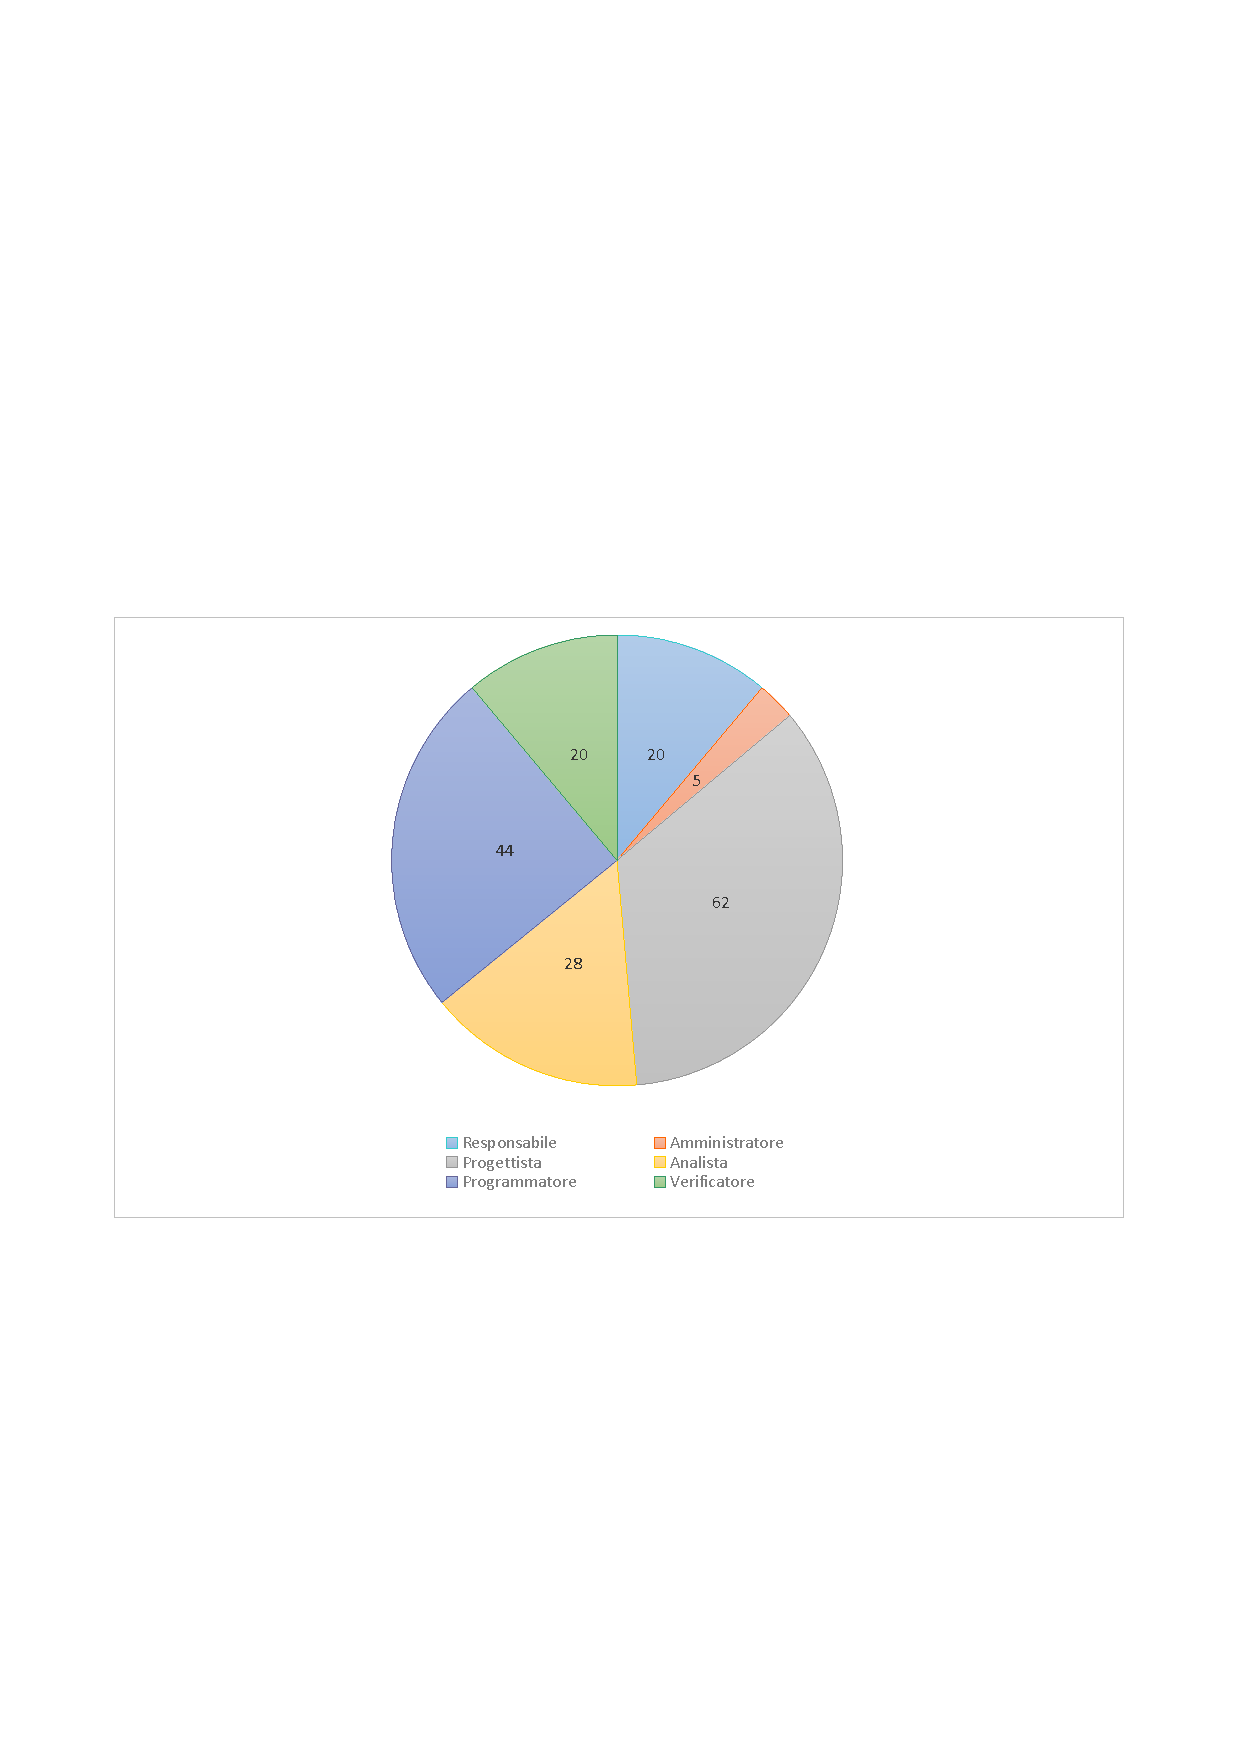
\includegraphics[width=0.93\textwidth , trim=1.5cm 9cm 1.5cm 9cm]{grafici/PDROB/PDROB-ore-ruolo}
			\caption{Fase PDROB - Ore per ruolo}
		\label{fig:CircleChart-fasePDROB_ore_r}
	\end{figure}

\vfill	
	\begin{figure}[H]
		\centering
		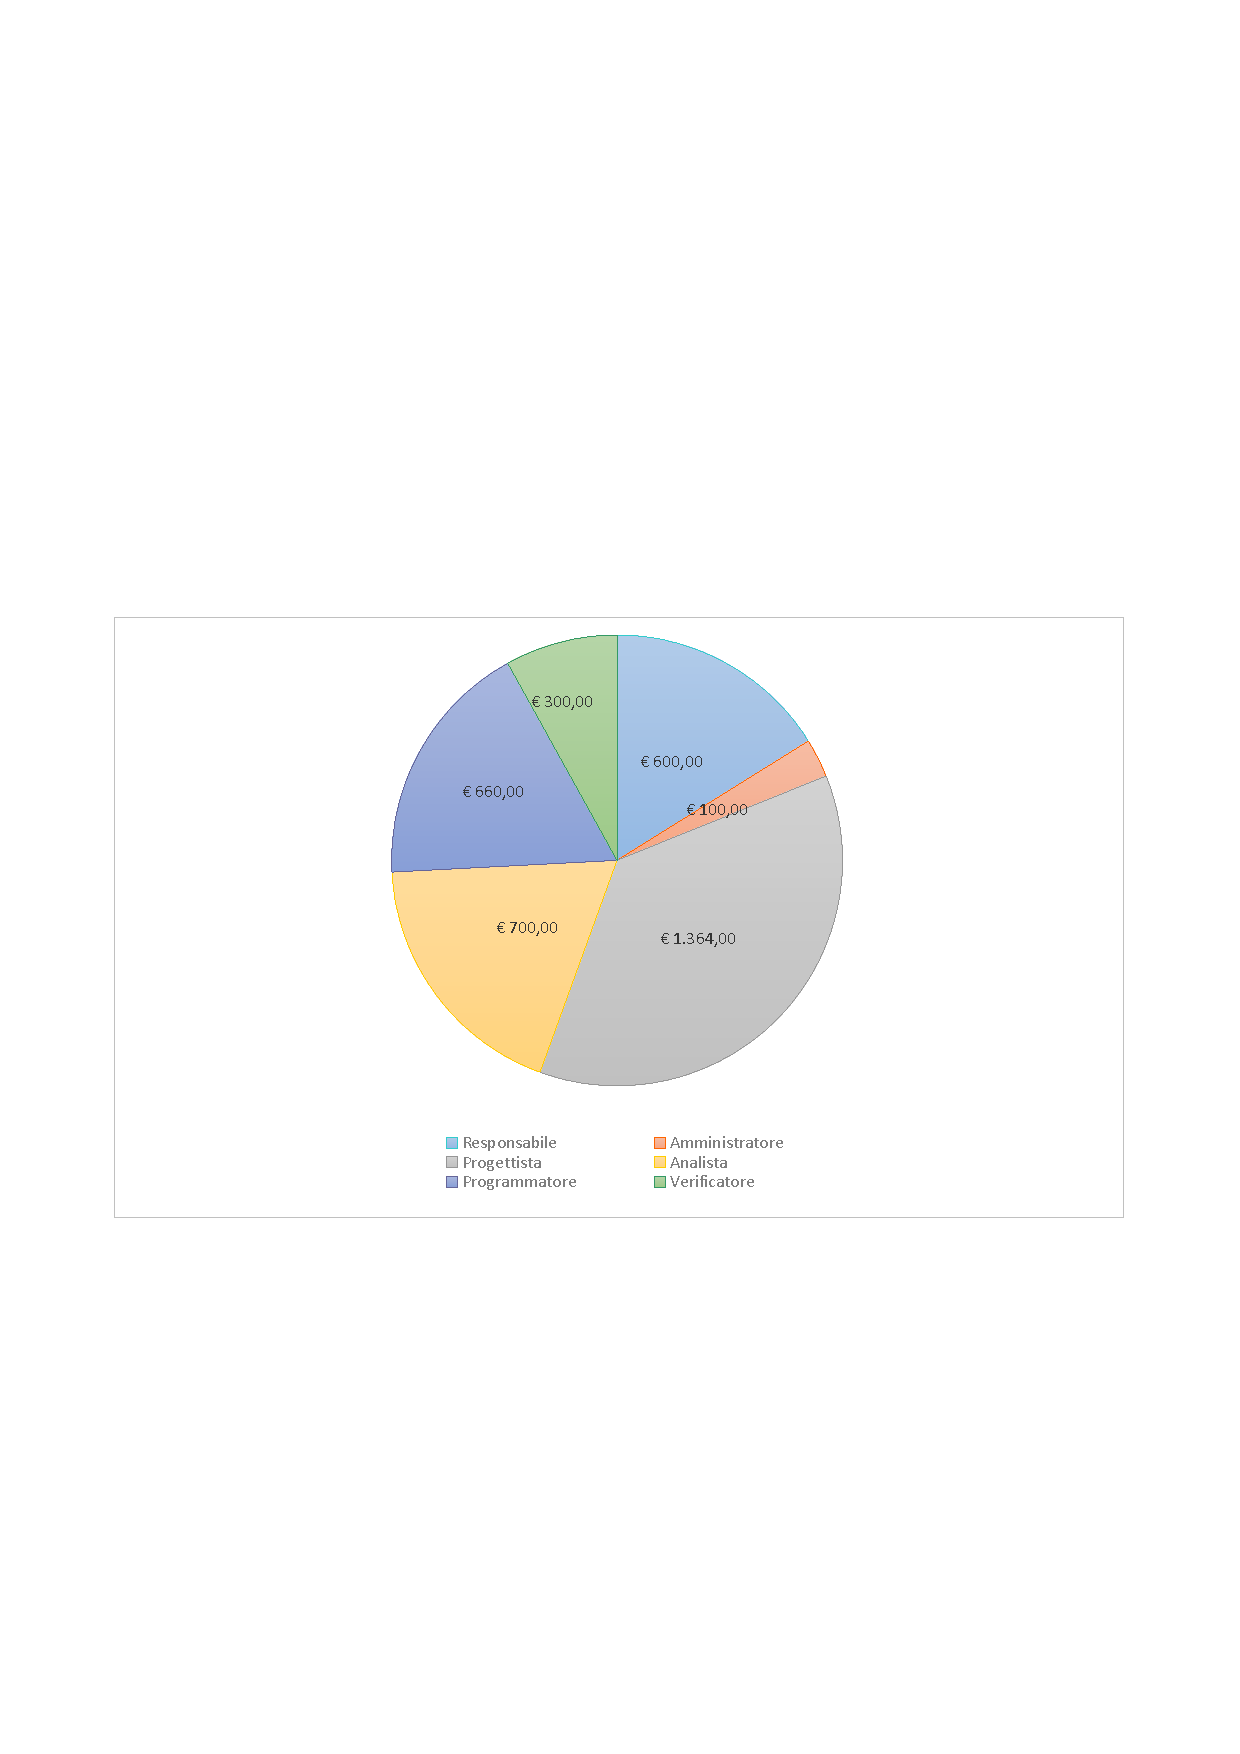
\includegraphics[width=0.93\textwidth , trim=1.5cm 9cm 1.5cm 9cm]{grafici/PDROB/PDROB-costo}
			\caption{Fase PDROB - Costo per ruolo}
		\label{fig:CircleChart-fasePDROB_costo}
	\end{figure}
\vfill	
\newpage	
	
	\subsubsection{Fase PDRD}
				\paragraph{Suddivisione del lavoro}\
						
	\begin{table}[H]
		%\centering
	
		\begin{tabularx}{\textwidth}{l  * {6}{C}  c}
			\toprule
			\textbf{Nominativo} & \textbf{Rp} & \textbf{Am} & \textbf{Pt} 
						& \textbf{An} & \textbf{Pm} & \textbf{Ve} & \textbf{Ore totali} \\
			\midrule
			Andrighetto Cristian  & 0 & 0 & 0 & 3 & 2 & 9 & 14 \\
			Bicego Eduard  & 0 & 9 & 0 & 2 & 0 & 3 & 14 \\
			Castello Davide  & 5 & 0 & 0 & 0 & 0 & 10 & 15 \\
			Conti Oscar Elia  & 0 & 0 & 0 & 0 & 10 & 5 & 15 \\
			Tavella Federico  & 0 & 0 & 0 & 0 & 8 & 7 & 15 \\
			Tombolato Andrea  & 0 & 0 & 5 & 4 & 0 & 6 & 15 \\
			Zanella Marco & 0 & 0 & 5 & 4 & 0 & 7 & 16 \\
			\midrule
			\textbf{Ore Totali Ruolo} & 5 & 9 & 10 & 13 & 20 & 47 & 104 \\
			\bottomrule
			
		\end{tabularx}
		\caption{Fase PDRD - Suddivisione delle ore di lavoro}
		\label{tab:fasePDRD_ore}
	\end{table}
\vfill	
		
	\begin{figure}[H]
		\centering
		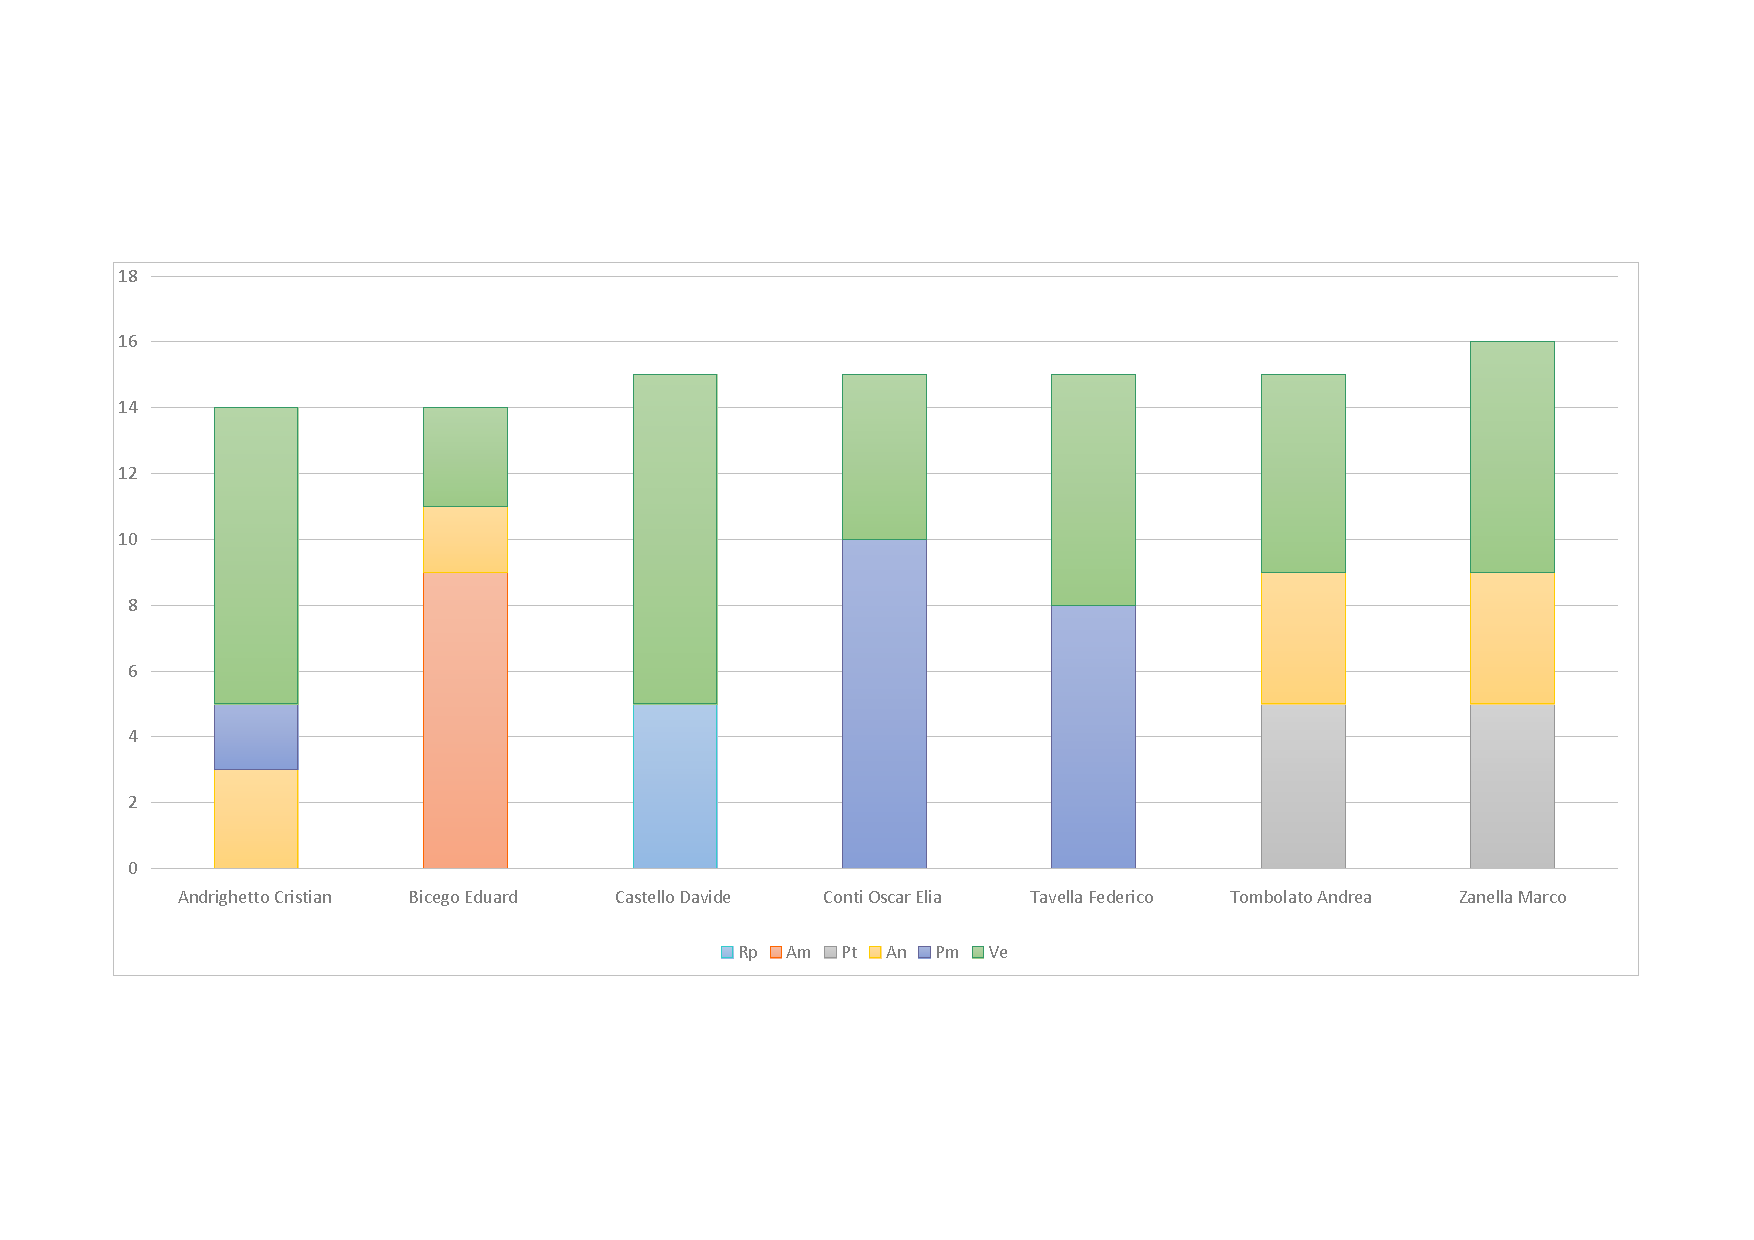
\includegraphics[width=\textwidth , trim=2cm 4cm 2cm 4cm]{grafici/PDRD/PDRD-ore-persona}
			\caption{Fase PDRD - Riassunto}
		\label{fig:BarChart-fasePDRD_ore}
	\end{figure}
\vfill	
\newpage	
	
	\paragraph{Prospetto economico}\
					
	\begin{table}[H]
		\centering
	
		\begin{tabular}{l * {2}{c}}
			\toprule
			\textbf{Ruolo} & \textbf{Ore} & \textbf{Costo (\euro{})} \\
			\midrule
			Responsabile & 5 & 150,00 \\
			Amministratore  & 9 & 180,00 \\
			Progettista  & 10 & 220,00 \\
			Analista & 13 & 325,00 \\
			Programmatore  & 20 & 300,00 \\
			Verificatore  & 47 & 705,00 \\
			\midrule
			\textbf{Totale}  & 104 & 1.880,00 \\
			\bottomrule
		\end{tabular}
		\caption{Fase PDRD - Costo per ruolo}
		\label{tab:fasePDRD_costo}
	\end{table}
\vfill	
	
	\begin{figure}[H]
		\centering
		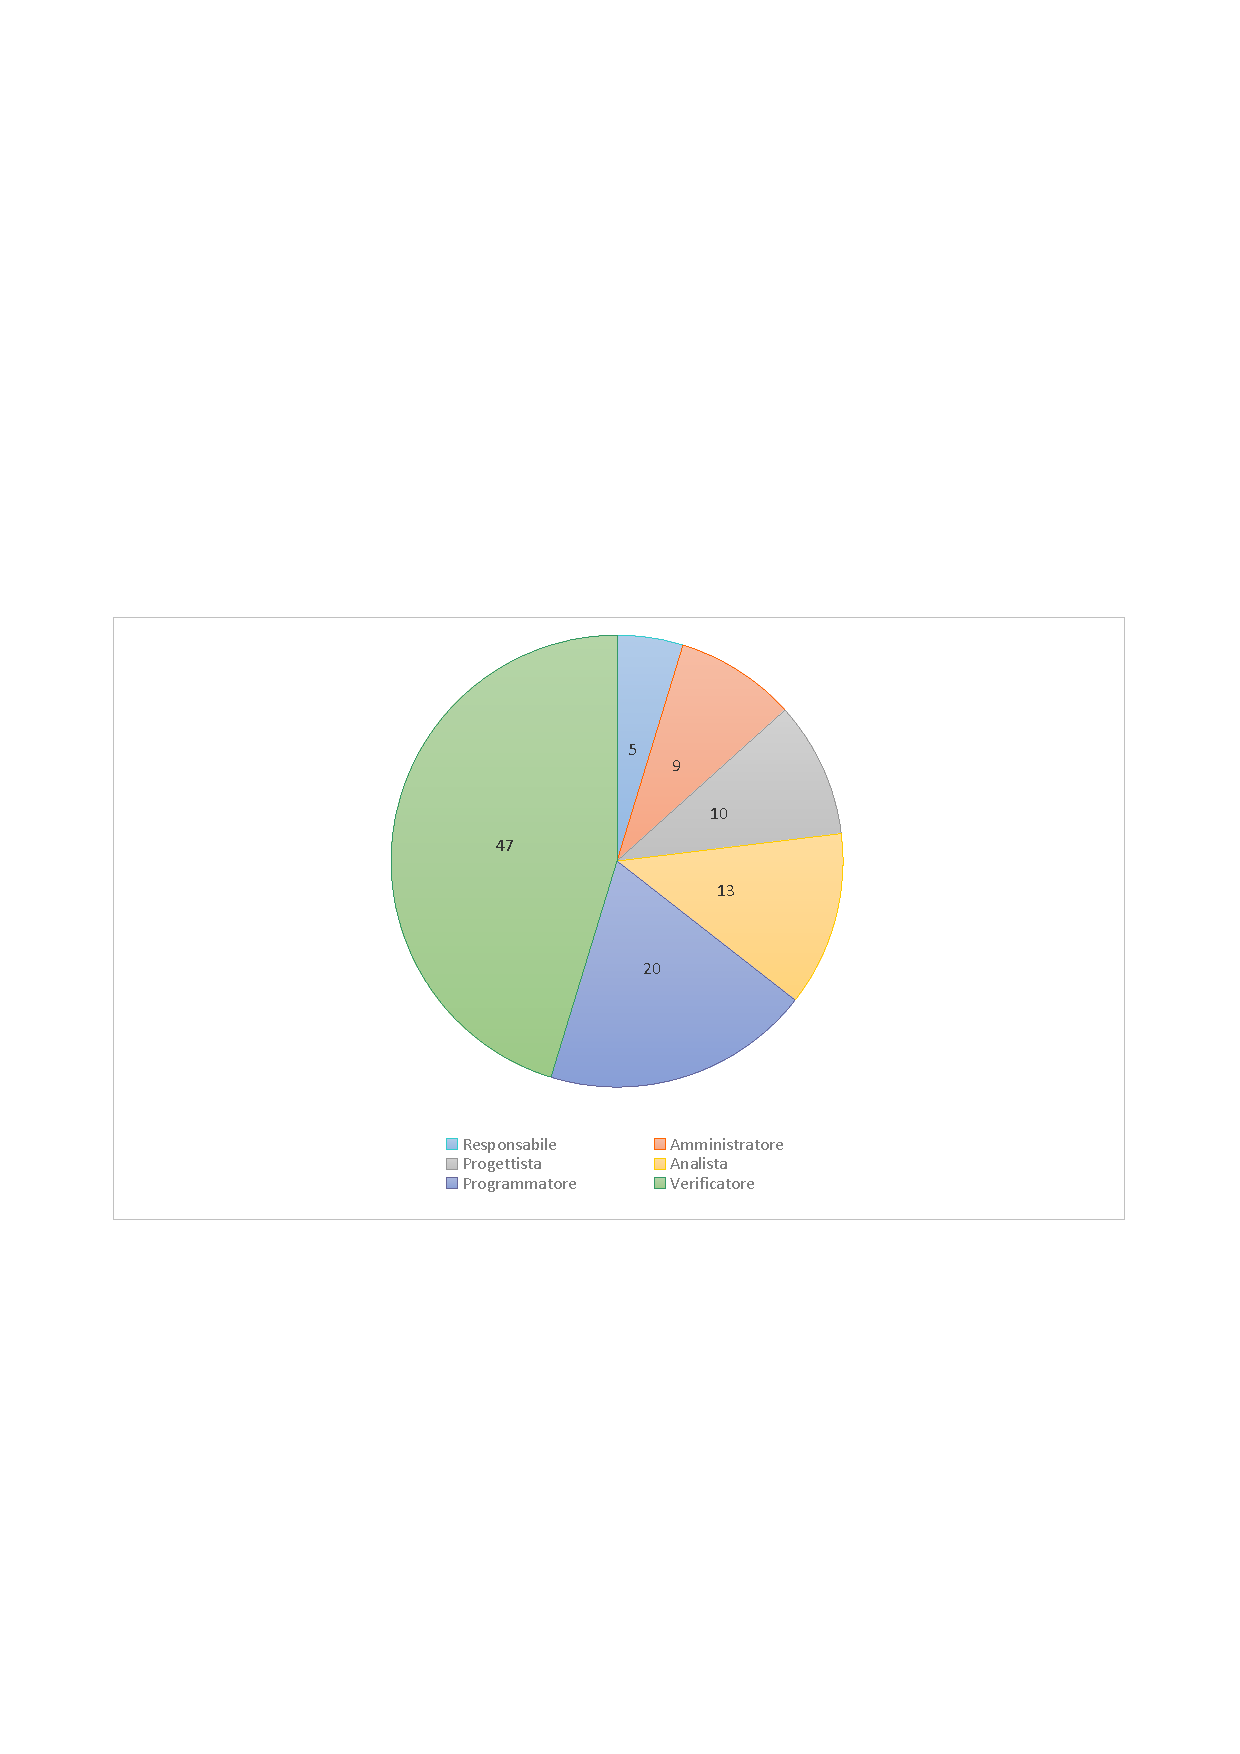
\includegraphics[width=0.93\textwidth , trim=1.5cm 9cm 1.5cm 9cm]{grafici/PDRD/PDRD-ore-ruolo}
			\caption{Fase PDRD - Ore per ruolo}
		\label{fig:CircleChart-fasePDRD_ore_r}
	\end{figure}
\vfill	
\newpage
\vfill
	\begin{figure}[H]
		\centering
		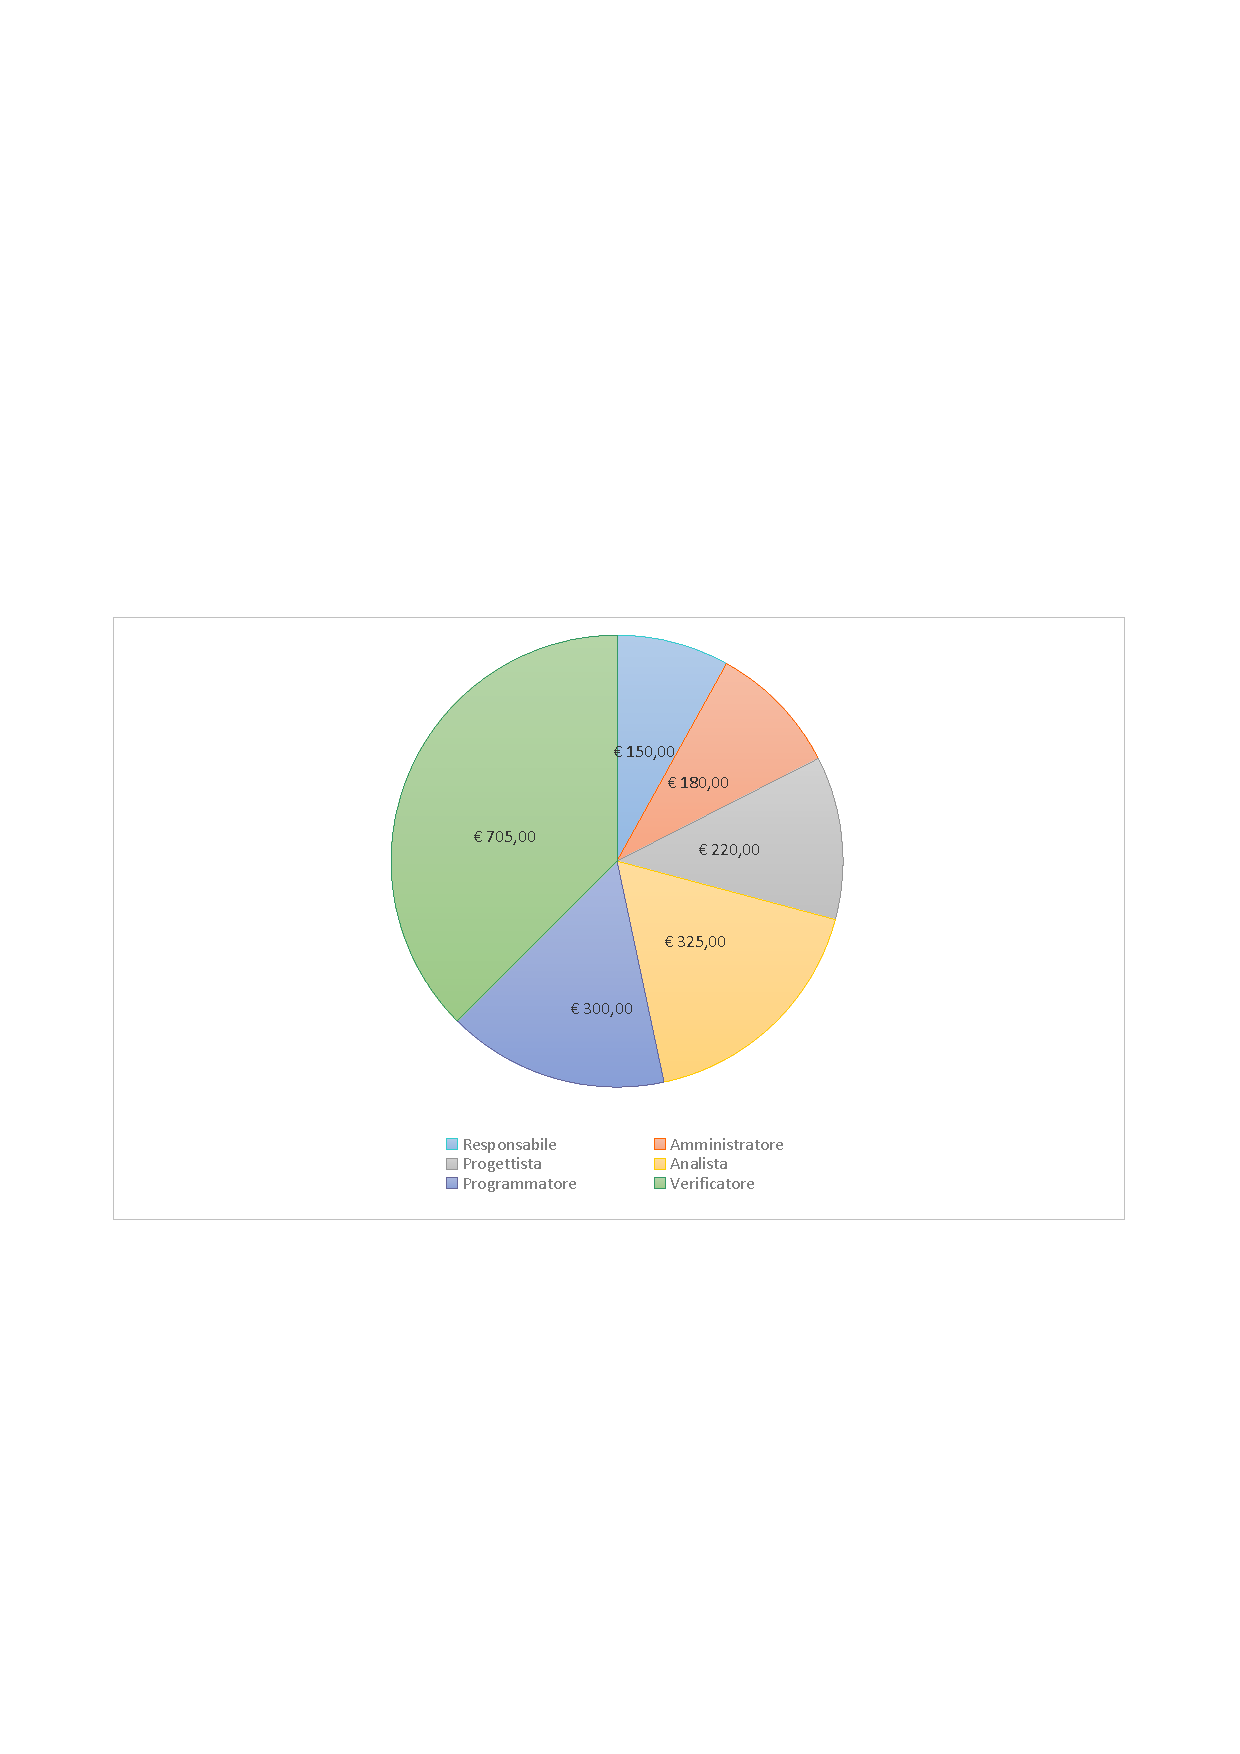
\includegraphics[width=0.93\textwidth , trim=1.5cm 9cm 1.5cm 9cm]{grafici/PDRD/PDRD-costo}
			\caption{Fase PDRD - Costo per ruolo}
		\label{fig:CircleChart-fasePDRD_costo_r}
	\end{figure}
\vfill
	
	\subsubsection{Fase PDROP}
				\paragraph{Suddivisione del lavoro}\
						
	\begin{table}[H]
		%\centering
		\begin{tabularx}{\textwidth}{l  * {6}{C}  c}
			\toprule
			\textbf{Nominativo} & \textbf{Rp} & \textbf{Am} & \textbf{Pt} 
						& \textbf{An} & \textbf{Pm} & \textbf{Ve} & \textbf{Ore totali} \\
			\midrule
			Andrighetto Cristian  & 0 & 0 & 0 & 0 & 3 & 10 & 13 \\
			Bicego Eduard  & 9 & 0 & 3 & 0 & 2 & 0 & 14 \\
			Castello Davide  & 0 & 0 & 6 & 0 & 0 & 6 & 12 \\
			Conti Oscar Elia  & 0& 9 & 0 & 6 & 0 & 0 & 15 \\
			Tavella Federico  & 0 & 0 & 7 & 0 & 0 & 5 & 12 \\
			Tombolato Andrea  & 0 & 0 & 0 & 11 & 3 & 0 & 14 \\
			Zanella Marco & 0 & 12 & 0 & 3 & 0 & 0 & 15 \\
			\midrule
			\textbf{Ore Totali Ruolo} & 9 & 21 & 16 & 20 & 8 & 21 & 95 \\
			\bottomrule
			
		\end{tabularx}
		\caption{Fase PDROP - Suddivisione delle ore di lavoro}
		\label{tab:fasePDROP_ore}
	\end{table}
	
\newpage
\vfill	
		
	\begin{figure}[H]
		\centering
		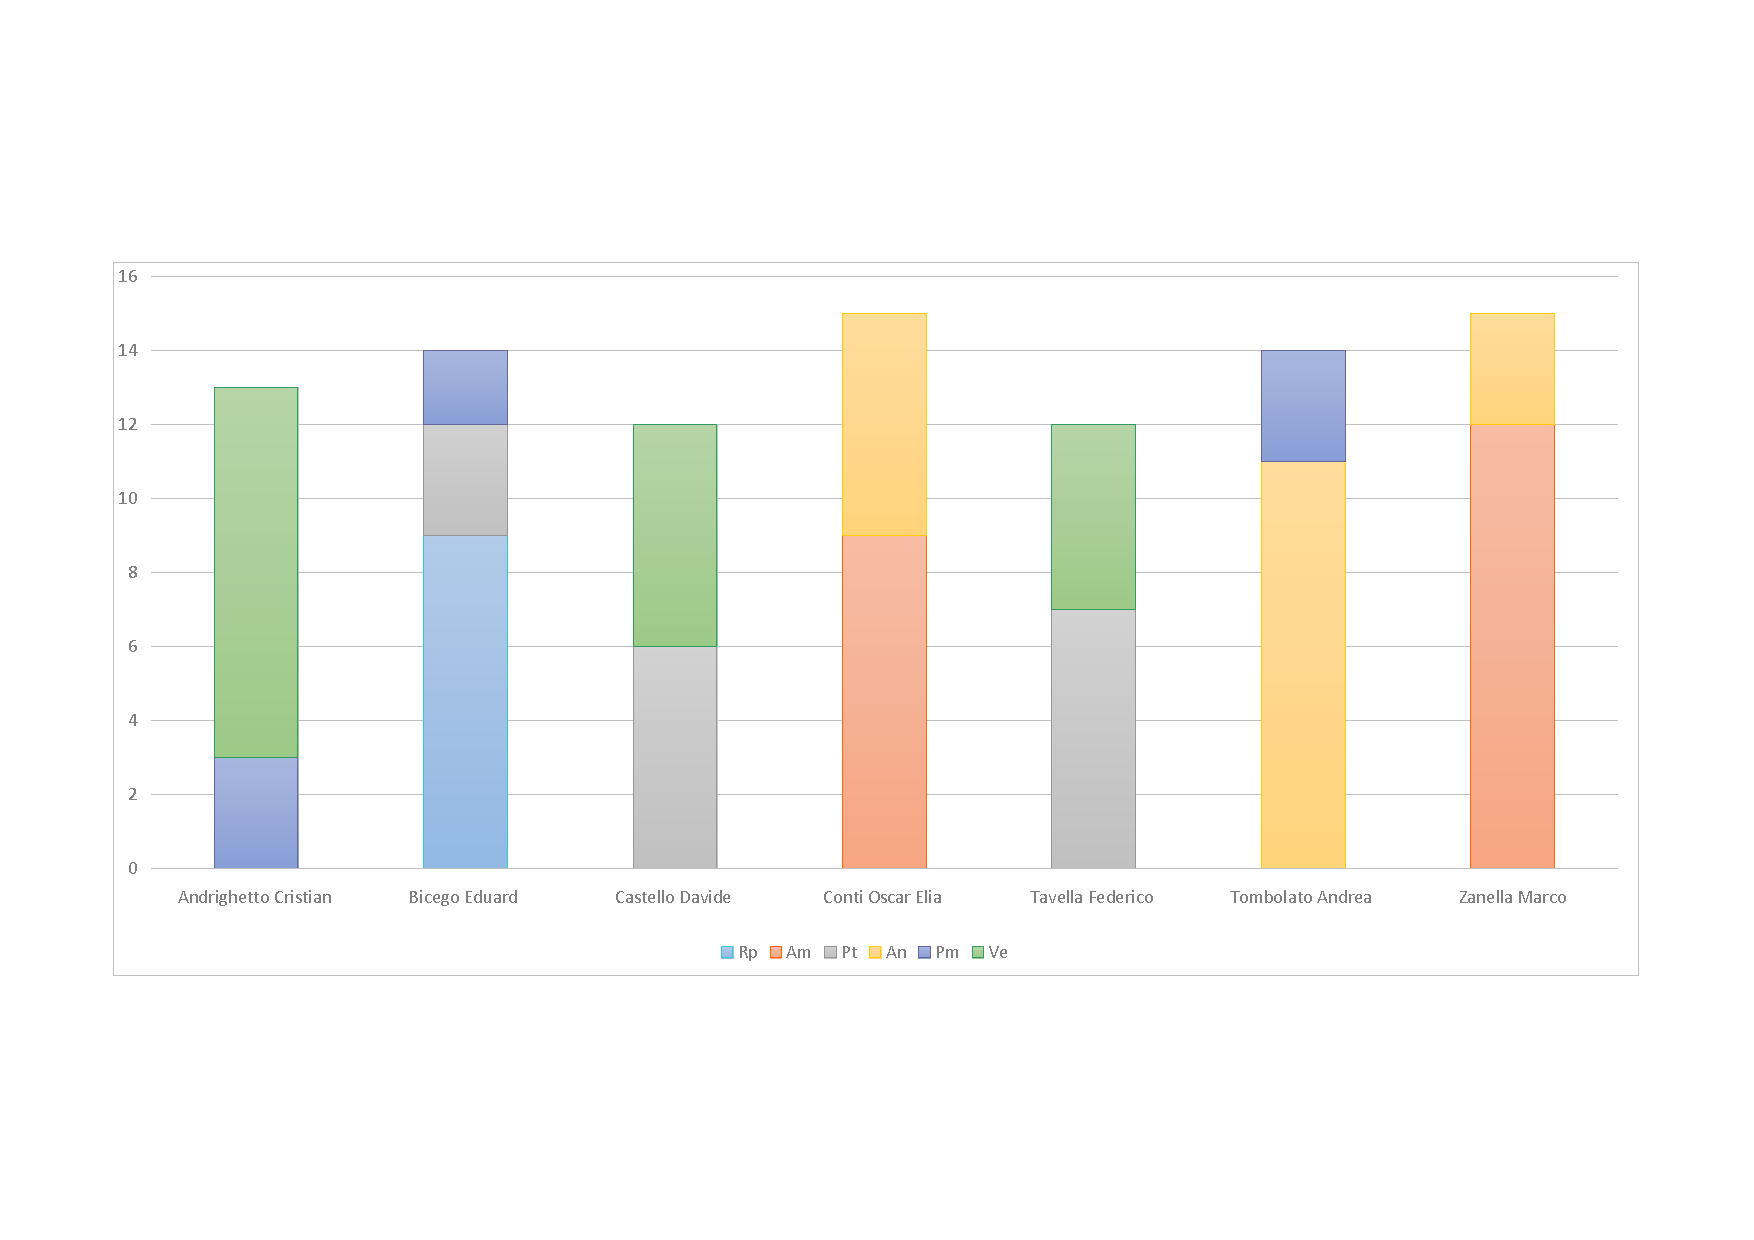
\includegraphics[width=\textwidth , trim=2cm 4cm 2cm 4cm]{grafici/PDROP/PDROP-ore-persona}
			\caption{Fase PDROP - Riassunto}
		\label{fig:BarChart-fasePDROP_ore}
	\end{figure}
\vfill	
	
	\paragraph{Prospetto economico}\
					
	\begin{table}[H]
		\centering
	
		\begin{tabular}{l * {2}{c}}
			\toprule
			\textbf{Ruolo} & \textbf{Ore} & \textbf{Costo (\euro{})} \\
			\midrule
			Responsabile & 9     &  270,00 \\
			Amministratore  & 21    &  420,00 \\
			Progettista  & 16   &  352,00 \\
			Analista & 20    &  500,00 \\
			Programmatore  & 8    &  120,00 \\
			Verificatore  & 21    &  315,00 \\
			\midrule
			\textbf{Totale}  & 95   &  1.977,00 \\
			\bottomrule
		\end{tabular}
		\caption{Fase PDROP - Costo per ruolo}
		\label{tab:fasePDROP_costo}
	\end{table}
\vfill	
\newpage
\vfill	
	
	\begin{figure}[H]
		\centering
		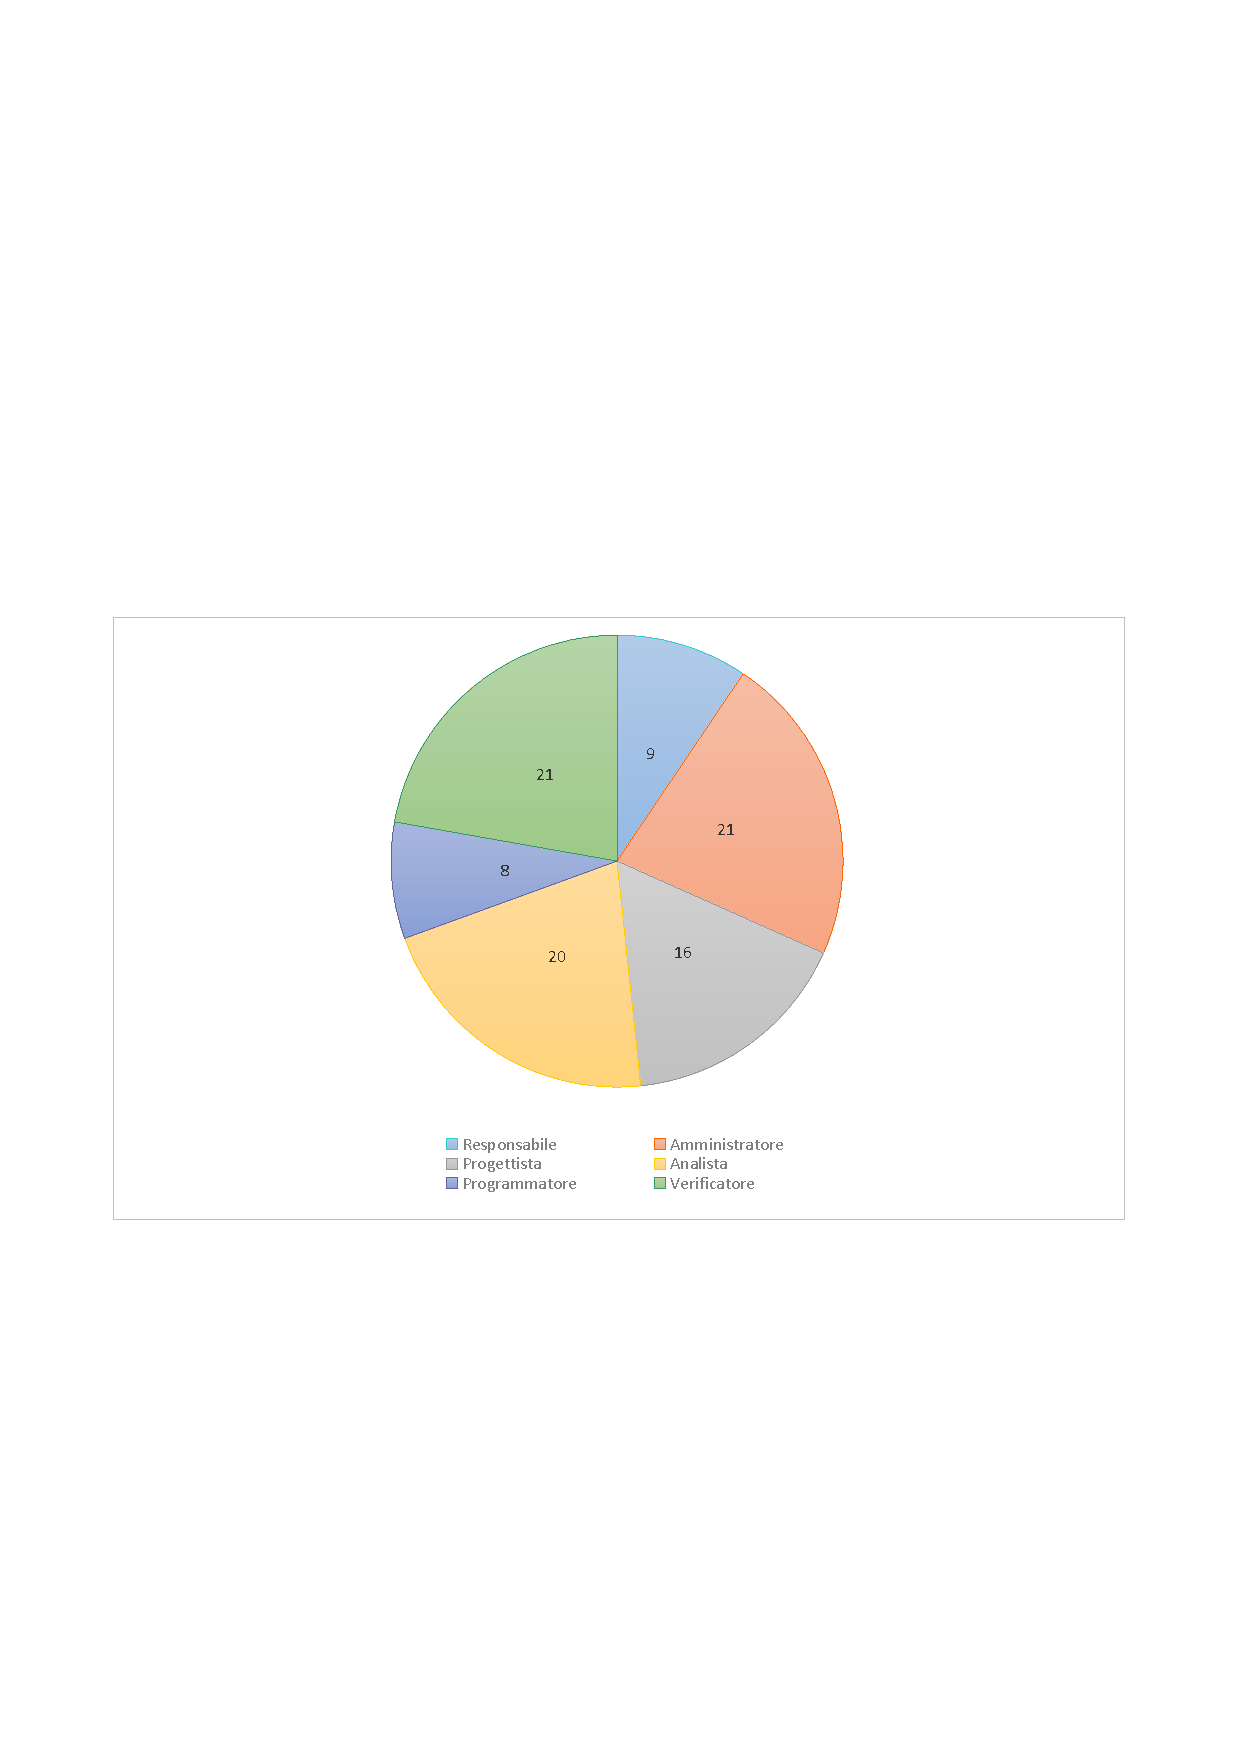
\includegraphics[width=0.93\textwidth , trim=1.5cm 9cm 1.5cm 9cm]{grafici/PDROP/PDROP-ore-ruolo}
			\caption{Fase PDROP - Ore per ruolo}
		\label{fig:CircleChart-fasePDROP_ore_r}
	\end{figure}
\vfill
	\begin{figure}[H]
		\centering
		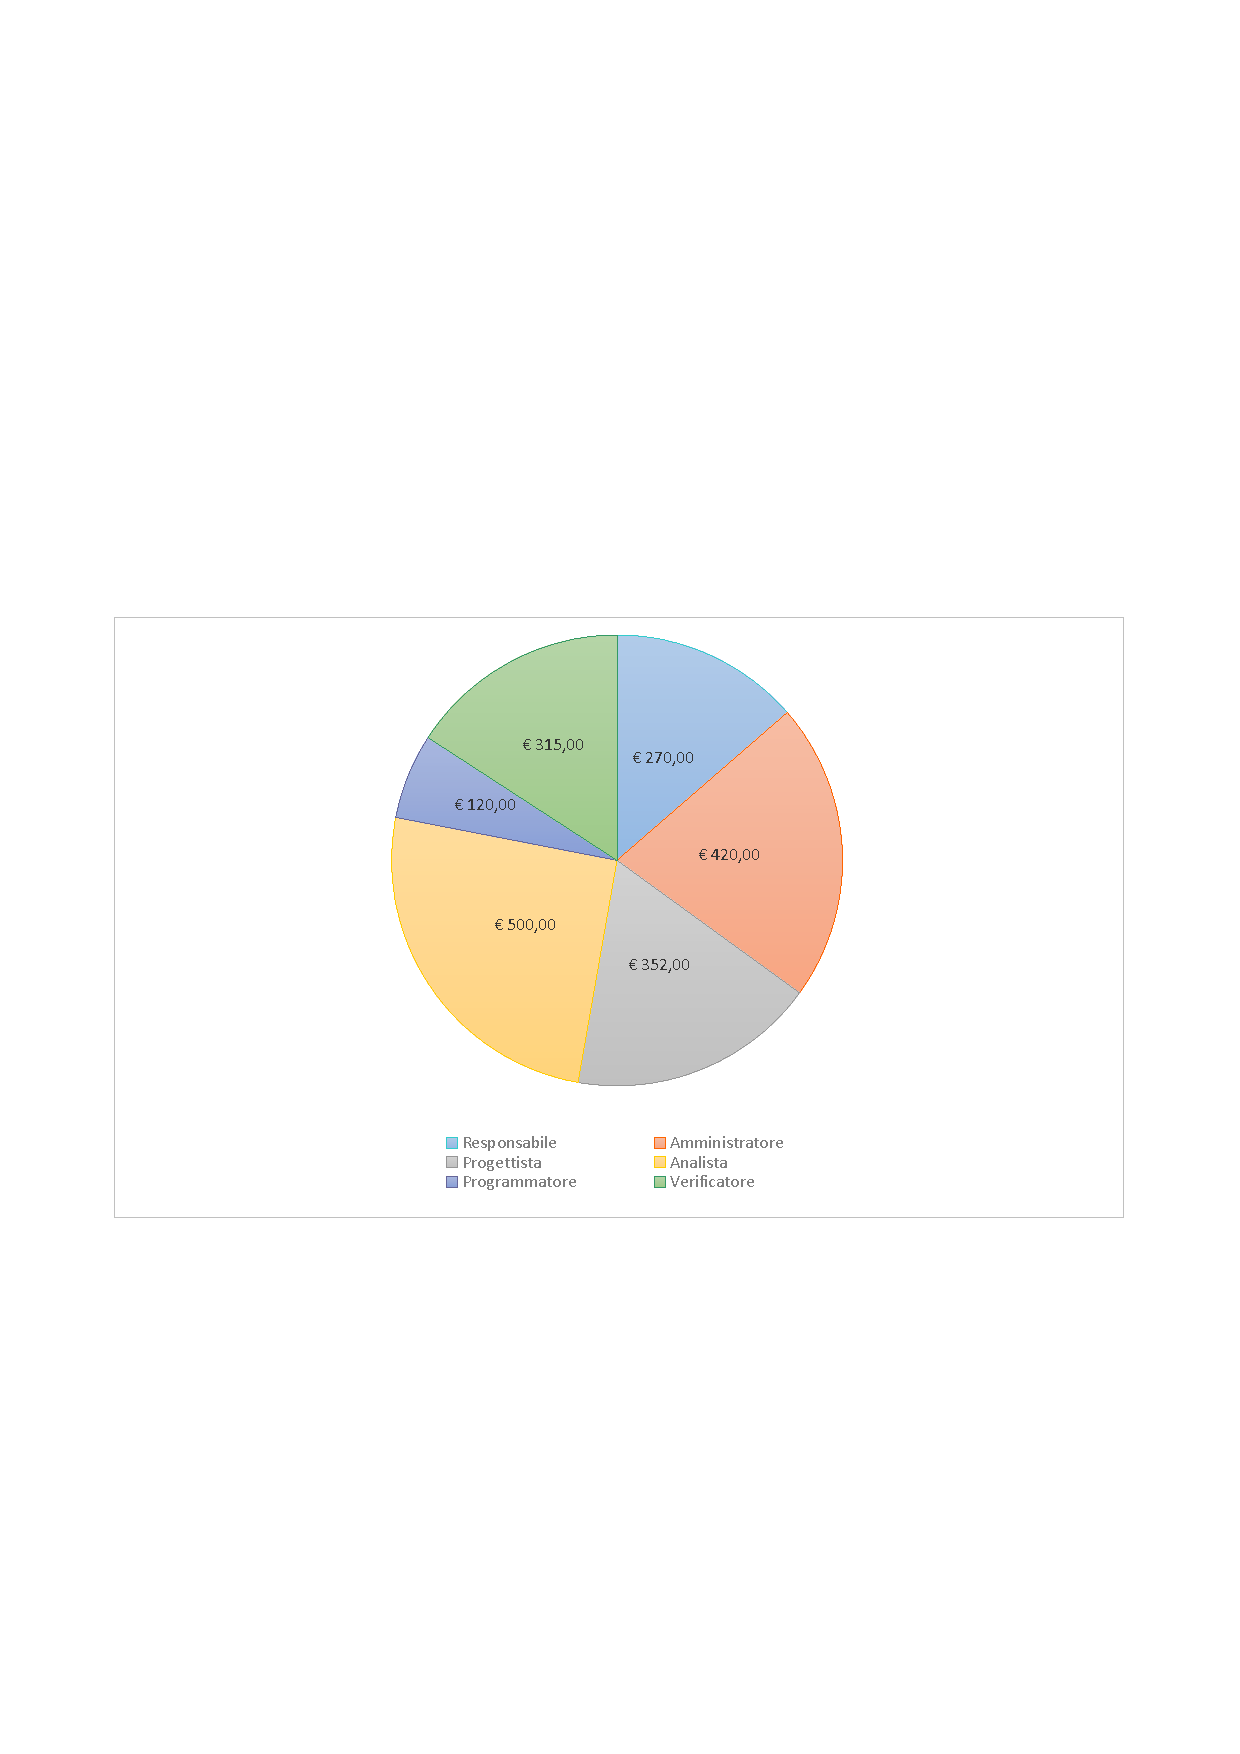
\includegraphics[width=0.93\textwidth , trim=1.5cm 9cm 1.5cm 9cm]{grafici/PDROP/PDROP-costo}
			\caption{Fase PDROP - Costo per ruolo}
		\label{fig:CircleChart-fasePDROP_costo}
	\end{figure}
\vfill	
\newpage
	
	\subsubsection{Fase V}
				\paragraph{Suddivisione del lavoro}\
					
	\begin{table}[H]
		%\centering
		\begin{tabularx}{\textwidth}{l  * {6}{C}  c}
			\toprule
			\textbf{Nominativo} & \textbf{Rp} & \textbf{Am} & \textbf{Pt} 
						& \textbf{An} & \textbf{Pm} & \textbf{Ve} & \textbf{Ore totali} \\
			\midrule
			Andrighetto Cristian  & 0 & 4 & 0 & 0 & 0 & 11 & 15 \\
			Bicego Eduard  & 0 & 0 & 0 & 0 & 9 & 6 & 15 \\
			Castello Davide  & 0 & 0 & 0 & 0 & 9 & 6 & 15 \\
			Conti Oscar Elia  & 0 & 11& 0 & 0 & 0 & 5 & 16 \\
			Tavella Federico  & 0 & 0 & 0 & 0 & 0 & 16 & 16 \\
			Tombolato Andrea  & 10 & 0 & 0 & 0 & 4 & 2 & 16 \\
			Zanella Marco & 0 & 0 & 7 & 0 & 0 & 9 & 16 \\
			\midrule
			\textbf{Ore Totali Ruolo} & 10 & 15 & 7 & 0 & 22 & 55 & 109 \\
			\bottomrule
		\end{tabularx}
		\caption{Fase V - Suddivisione delle ore di lavoro}
		\label{tab:faseV_ore}
	\end{table}
\vfill	

	
	\begin{figure}[H]
		\centering
		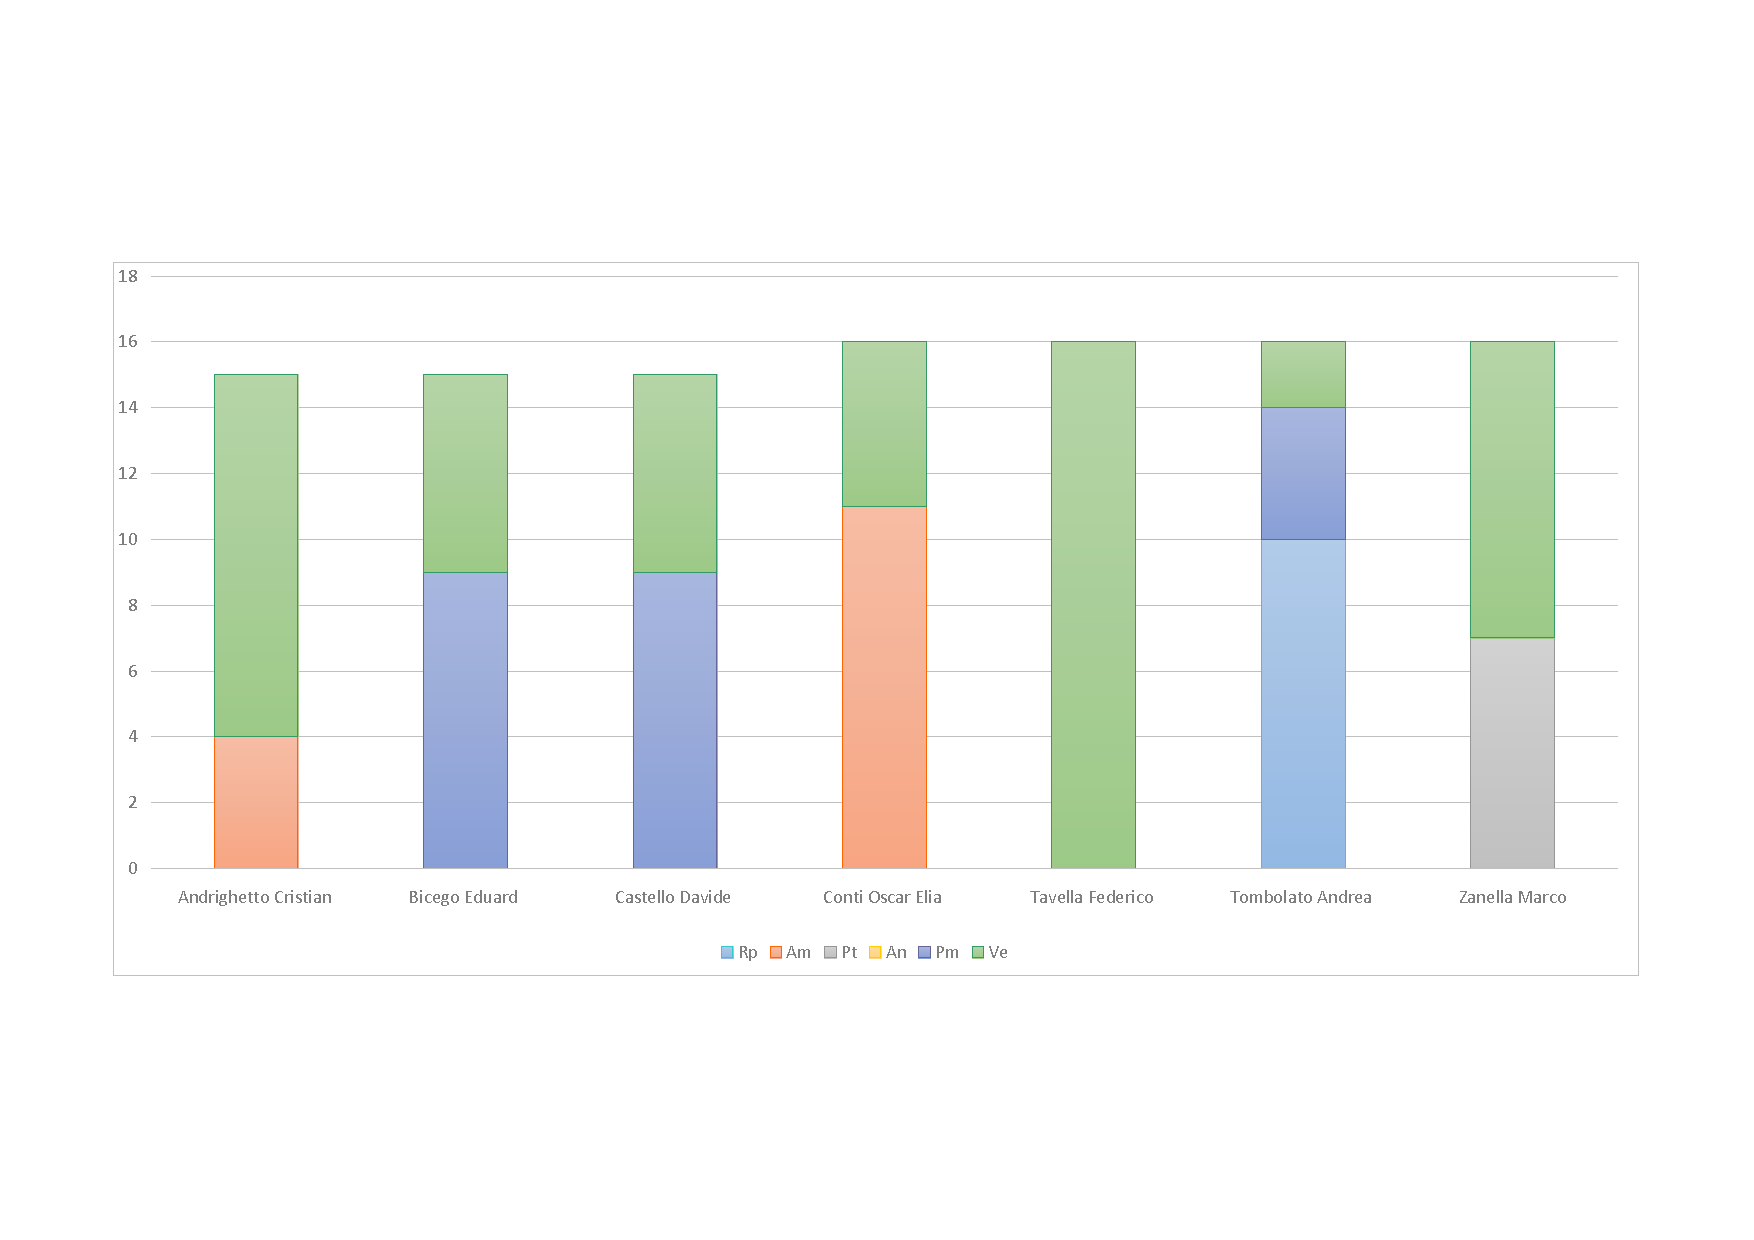
\includegraphics[width=\textwidth , trim=2cm 4cm 2cm 4cm]{grafici/V/V-ore-persona}
			\caption{Fase V - Riassunto}
		\label{fig:BarChart-faseV_ore}
	\end{figure}
\vfill	
\newpage
\vfill
	\paragraph{Prospetto economico}\
					
	\begin{table}[H]
		\centering
	
		\begin{tabular}{l * {2}{c}}
			\toprule
			\textbf{Ruolo} & \textbf{Ore} & \textbf{Costo (\euro{})} \\
			\midrule
			Responsabile & 10 & 300,00 \\
			Amministratore  & 15 & 300,00 \\
			Progettista  & 7 & 154,00 \\
			Analista & 0 & 0,00 \\
			Programmatore  & 22 &  330,00 \\
			Verificatore  & 55 &  825,00 \\
			\midrule
			\textbf{Totale}  & 109   &  1.909,00 \\
			\bottomrule	
		\end{tabular}
		\caption{Fase V - Costo per ruolo}
		\label{tab:faseV_costo}
	\end{table}
\vfill	
	
	\begin{figure}[H]
		\centering
		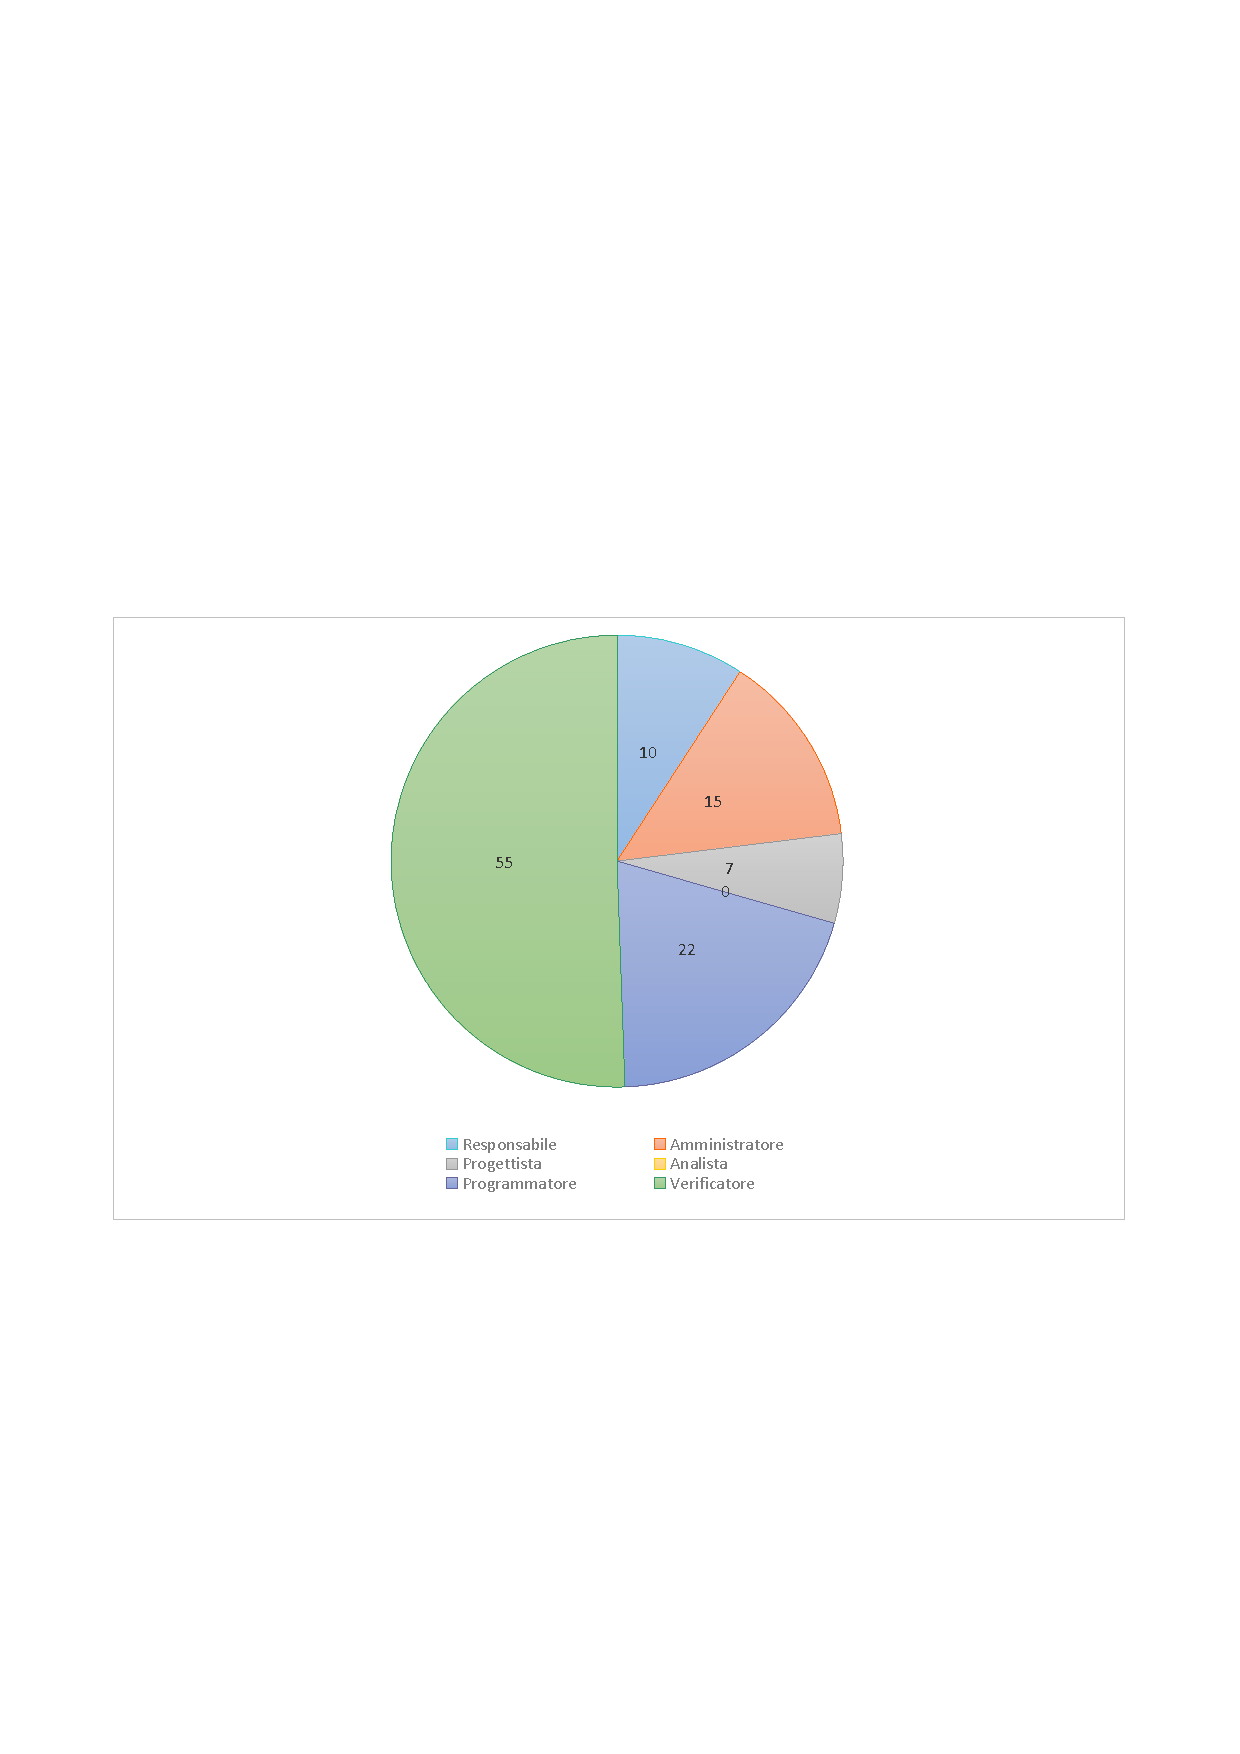
\includegraphics[width=0.93\textwidth , trim=1.5cm 9cm 1.5cm 9cm]{grafici/V/V-ore-ruolo}
			\caption{Fase V - Ore per ruolo}
		\label{fig:CircleChart-faseV_ore_r}
	\end{figure}
\vfill	
\newpage
	\begin{figure}[H]
		\centering
		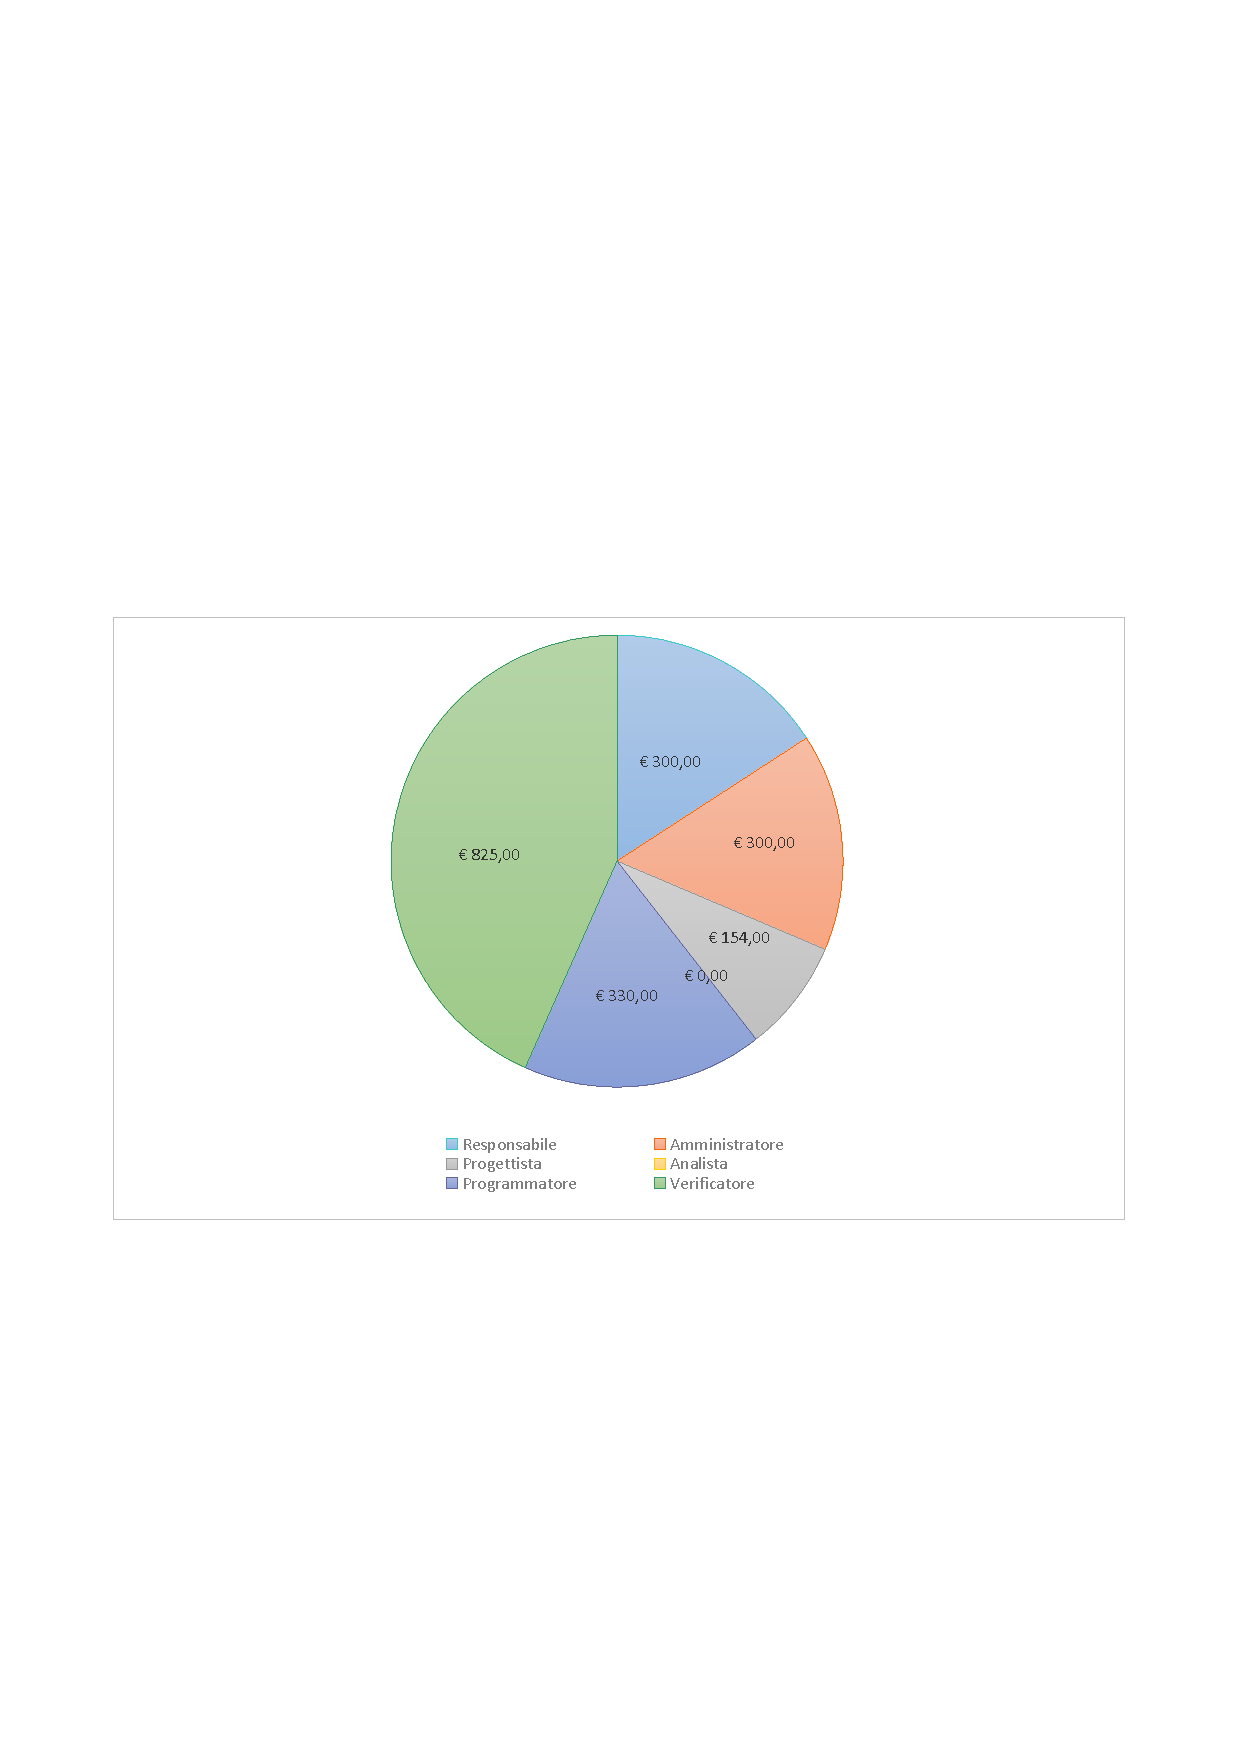
\includegraphics[width=0.93\textwidth , trim=1.5cm 9.5cm 1.5cm 9cm]{grafici/V/V-costo}
			\caption{Fase V - Costo per ruolo}
		\label{fig:CircleChart-faseV_costo}
	\end{figure}	
	
	\subsection{Riepilogo}
			\subsubsection{Ore totali}
				\paragraph{Suddivisione del lavoro}\
					Le ore totali che ogni componente del gruppo \leaf\ dedicherà ad ognuno dei ruoli, a rotazione, sono indicate di seguito:
	
	\begin{table}[H]
		%\centering
		\begin{tabularx}{\textwidth}{l  * {6}{C}  c}
			\toprule
			\textbf{Nominativo} & \textbf{Rp} & \textbf{Am} & \textbf{Pt} 
						& \textbf{An} & \textbf{Pm} & \textbf{Ve} & \textbf{Ore totali} \\
			\midrule
			Andrighetto Cristian  & 9  & 22 & 18 & 38 & 7  & 56 & 150 \\
			Bicego Eduard  & 13 & 25 & 23 & 20 & 25 & 47 & 153 \\
			Castello Davide  & 5  & 30 & 28 & 36 & 9  & 43 & 151 \\
			Conti Oscar Elia  & 10 & 40 & 22 & 37 & 18 & 26 & 153 \\
			Tavella Federico  & 27 & 12 & 23 & 37 & 20 & 35 & 154 \\
			Tombolato Andrea  & 22 & 15 & 25 & 39 & 23 & 31 & 155 \\
			Zanella Marco & 10 & 27 & 24 & 35 & 12 & 41 & 149 \\
			\midrule
			\textbf{Ore Totali Ruolo} & 96    & 171   & 163   & 242   & 114   & 279   & 1065 \\
			\bottomrule
		\end{tabularx}
		\caption{Ore totali - Suddivisione delle ore di lavoro}
		\label{tab:totale_ore}
	\end{table}
	
\newpage
\vfill
		
	\begin{figure}[H]
		\centering
		\includegraphics[width=\textwidth , trim=2cm 4cm 2cm 4cm]{grafici/Riepilogo/Totali/ore-persona}
			\caption{Ore persona totali - Riassunto}
		\label{fig:BarChart-totale_ore}
	\end{figure}
	
\vfill	
	
	\paragraph{Prospetto economico}\
					Il costo totale per ogni ruolo, comprensivo sia delle ore di formazione (a carico del gruppo \leaf) sia delle ore rendicontate (a carico del proponente), è dunque il seguente:
	\begin{table}[H]
		\centering
		\begin{tabular}{l * {2}{c}}
			\toprule
			\textbf{Ruolo} & \textbf{Ore} & \textbf{Costo (\euro{})} \\
			\midrule
			Responsabile & 96    &  2.880,00 \\
			Amministratore  & 171   &  3.420,00 \\
			Progettista  & 163   &  3.586,00 \\
			Analista & 242   &  6.050,00 \\
			Programmatore  & 114   &  1.710,00 \\
			Verificatore  & 279   &  4.185,00 \\
			\midrule
			\textbf{Totale}  & 1065  &  21.831,00 \\
			\bottomrule
			
		\end{tabular}
		\caption{Ore totali - Costo per ruolo}
		\label{tab:totale_costo}
	\end{table}
\vfill
\newpage	
\vfill
	
	\begin{figure}[H]
		\centering
		\includegraphics[width=0.93\textwidth , trim=1.5cm 9cm 1.5cm 9cm]{grafici/Riepilogo/Totali/ore-ruolo}
			\caption{Ore totali - Ore per ruolo}
		\label{fig:CircleChart-totale_ore_r}
	\end{figure}	
\vfill
	\begin{figure}[H]
		\centering
		\includegraphics[width=0.93\textwidth , trim=1.5cm 9cm 1.5cm 9cm]{grafici/Riepilogo/Totali/costo}
			\caption{Ore totali - Costo per ruolo}
		\label{fig:CircleChart-totale_ore}
	\end{figure}
\vfill
\newpage
	
	\subsubsection{Ore di investimento}
				\paragraph{Suddivisione del lavoro}\
					Le ore di investimento che ogni componente del gruppo \leaf\ dedicherà ad ognuno dei ruoli, a rotazione, vengono indicate di seguito:
	
	\begin{table}[H]
		%\centering
		\begin{tabularx}{\textwidth}{l  * {6}{C}  c}
			\toprule
			\textbf{Nominativo} & \textbf{Rp} & \textbf{Am} & \textbf{Pt} 
						& \textbf{An} & \textbf{Pm} & \textbf{Ve} & \textbf{Ore totali} \\
			\midrule
			Andrighetto Cristian  & 0     & 15    & 3     & 10    & 2     & 15    & 45 \\
			Bicego Eduard  & 4     & 10    & 3     & 0     & 5     & 26    & 48 \\
			Castello Davide  & 0     & 20    & 3     & 10    & 0     & 13    & 46 \\
			Conti Oscar Elia  & 0     & 20    & 3     & 15    & 5     & 5     & 48 \\
			Tavella Federico  & 17    & 3     & 3     & 21    & 5     & 0     & 49 \\
			Tombolato Andrea  & 12    & 5     & 4     & 20    & 3     & 6     & 50 \\
			Zanella Marco & 0     & 15    & 4     & 10    & 0     & 15    & 44 \\
			\midrule
			\textbf{Ore Totali Ruolo} & 33    & 88    & 23    & 86    & 20    & 80    & 330 \\
			\bottomrule
		\end{tabularx}
		\caption{Ore di investimento - Suddivisione delle ore di lavoro}
		\label{tab:investimento_ore}
	\end{table}
\vfill	

	
	\begin{figure}[H]
		\centering
		\includegraphics[width=\textwidth , trim=2cm 4cm 2cm 4cm]{grafici/Riepilogo/Investimento/ore-persona}
			\caption{Ore di investimento - Riassunto}
		\label{fig:BarChart-investimento_ore}
	\end{figure}
\vfill
\newpage
\vfill	
	\paragraph{Prospetto economico}\
					Il costo d'investimento per ogni ruolo è dunque il seguente:
	\begin{table}[H]
		\centering
		\begin{tabular}{l * {2}{c}}
			\toprule
			\textbf{Ruolo} & \textbf{Ore} & \textbf{Costo (\euro{})} \\
			\midrule
			Responsabile & 33    & 990,00 \\
			Amministratore  & 88    & 1.760,00 \\
			Progettista  & 23    & 506,00 \\
			Analista & 86    & 2.150,00 \\
			Programmatore  & 20    & 300,00 \\
			Verificatore  & 80    & 1.200,00 \\
			\midrule
			\textbf{Totale}  & 330   & 6.906,00 \\
			\bottomrule
		\end{tabular}
		\caption{Ore di investimento - Costo per ruolo}
		\label{tab:investimento_costo}
	\end{table}
\vfill	
	
	\begin{figure}[H]
		\centering
		\includegraphics[width=0.93\textwidth , trim=1.5cm 9cm 1.5cm 9cm]{grafici/Riepilogo/Investimento/ore-ruolo}
			\caption{Ore di investimento - Ore per ruolo}
		\label{fig:CircleChart-investimento_ore_r}
	\end{figure}
\vfill	
\newpage
	\begin{figure}[H]
		\centering
		\includegraphics[width=0.93\textwidth , trim=1.5cm 9cm 1.5cm 9cm]{grafici/Riepilogo/Investimento/costo}
			\caption{Ore di investimento - Costo per ruolo}
		\label{fig:CircleChart-investimento_costo}
	\end{figure}
\vfill	

	\subsubsection{Ore rendicontate}
				\paragraph{Suddivisione del lavoro}\
					Le ore rendicontate che ogni componente del gruppo \leaf\ dedicherà ad ognuno dei ruoli, a rotazione, vengono indicate di seguito:
	
	\begin{table}[H]
		%\centering
		\begin{tabularx}{\textwidth}{l  * {6}{C}  c}
			\toprule
			\textbf{Nominativo} & \textbf{Rp} & \textbf{Am} & \textbf{Pt} 
						& \textbf{An} & \textbf{Pm} & \textbf{Ve} & \textbf{Ore totali} \\
			\midrule
			Andrighetto Cristian & 9 & 7 & 15 & 28 & 5 & 41 &	105 \\
			%\midrule
			Bicego Eduard & 9 & 15 & 20 & 20 & 20 & 21 & 105 \\
			%\midrule
			Castello Davide & 5 & 10 & 25 & 26 & 9 & 30 & 105 \\
			%\midrule
			Conti Oscar Elia & 10 & 20 & 19 & 22 & 13 & 21 & 105 \\
			%\midrule
			Tavella Federico &	10 & 9 & 20 & 16 & 15 & 35 & 105 \\
			%\midrule
			Tombolato Andrea & 10 & 10 & 21 & 19 & 20 & 25 & 105 \\
			%\midrule
			Zanella Marco & 10 & 12 & 20 & 25 & 12 & 26 & 105 \\
			\midrule			
			\textbf{Ore Totali Ruolo} & 63 & 83 & 140 & 156 & 94 & 199 & 735 \\
			\bottomrule
		\end{tabularx}
		\caption{Ore rendicontate - Suddivisione delle ore di lavoro}
		\label{tab:rendicontate_ore}
	\end{table}
	
\newpage
\vfill		
	
	\begin{figure}[H]
		\centering
		\includegraphics[width=\textwidth , trim=2cm 4cm 2cm 4cm]{grafici/Riepilogo/Rendicontate/ore-persona}
			\caption{Ore rendicontate - Riassunto}
		\label{fig:BarChart-rendicontate_ore}
	\end{figure}
	
\vfill
	
	\paragraph{Prospetto economico}\
					Il costo rendicontato per ogni ruolo è dunque il seguente:
	\begin{table}[H]
		\centering
		\begin{tabular}{l * {2}{c}}
			\toprule
			\textbf{Ruolo} & \textbf{Ore} & \textbf{Costo (\euro{})} \\
			\midrule
			Responsabile &	63 & 1.890,00 \\
			%\midrule
			Amministratore & 83 & 1.660,00 \\
			%\midrule
			Progettista & 140 & 3.080,00 \\
			%\midrule
			Analista & 156 & 3.900,00 \\
			%\midrule
			Programmatore & 94 & 1.410,00 \\
			%\midrule
			Verificatore & 199 & 2.985,00 \\
			\midrule		
			\textbf{Totale} & 735 & 14.925,00 \\
			\bottomrule
		\end{tabular}
		\caption{Ore rendicontate - Costo per ruolo}
		\label{tab:rendicontate_costo}
	\end{table}
\vfill
\newpage
\vfill	
	
	\begin{figure}[H]
		\centering
		\includegraphics[width=0.93\textwidth , trim=1.5cm 9cm 1.5cm 9cm]{grafici/Riepilogo/Rendicontate/ore-ruolo}
			\caption{Ore rendicontate - Ore per ruolo}
		\label{fig:CircleChart-rendicontate_ore_r}
	\end{figure}
\vfill	
	\begin{figure}[H]
		\centering
		\includegraphics[width=0.93\textwidth , trim=1.5cm 9cm 1.5cm 9cm]{grafici/Riepilogo/Rendicontate/costo}
			\caption{Ore rendicontate - Costo per ruolo}
		\label{fig:CircleChart-rendicontate_costo}
	\end{figure}
\vfill			
\end{document}